% REMEMBER: You must not plagiarise anything in your report. Be extremely careful.

\documentclass{l4proj}

    
%
% put any additional packages here
\usepackage{siunitx}
\usepackage{float}
\usepackage{tabularx}
\usepackage{amsmath}
%

\begin{document}

%==============================================================================
%% METADATA
\title{Using Deep Learning to predict overall survival times for breast cancer from H\&E stained whole slide biopsy images}
\author{Anirbit Ghosh}
\date{September 14, 2022}

\maketitle

%==============================================================================
%% ABSTRACT
\begin{abstract}
    Current pathological practice to diagnose malignancy involves the manual identification and annotation of the extent of cancerous tumour cells in a biopsy slide image by a trained pathologist. This process is highly resource intensive and is subject to the interpretation variability between different readers leading to inconsistent outcomes. Therefore a Deep Learning based automated cancer detection system which can accurately and robustly identify the extent of malignancy from the digital whole slide image would be a highly desirable and potentially industry changing advancement. The subsequent step after the initial cancer diagnosis requires vast amounts of the patient's clinical data to be collected and processed in order to deliver a survival time prediction. The clinical data required to produce a survival time model for a patient ranges from general health and quality of life measures to specific characteristics of the malignant areas which must be extracted manually by pathologists. Given the sensitive nature of a cancer diagnosis in the first place it is often of essence to avoid putting patients through extensive diagnostic tests and data collection only to deliver potentially worse news with the survival time prognosis. Biopsy slide images hold a plethora of cellular level and structural information which can very effectively help understand the exact nature of malignancy. However, manually analyzing whole slide images to extract useful features is extremely expensive in terms of time and storage due to the sheer size of these images. Thus, augmenting the Deep Learning based cancer detection system to automatically extract useful features from the digital biopsy images can aid in characterizing cancer severity and giving a survival time estimate without the need of vast amounts of clinical data. The biggest problem in creating this system is the lack of annotated patient biopsy data that is publicly available, which makes effectively training a network to automatically detect malignant tissue extremely challenging. In this project, I proposed training a deep neural network on the Camelyon 16 data, which is a collection of 170 weakly annotated lymph node whole slide images from breast cancer patients. Breast cancer frequently metastasizes to axillary lymph nodes which makes them a good prognostic factor of breast cancer severity. The data contained 70 metastatic and 100 non-metastatic whole slides giving a good balance of positive and negative samples to train the network to accurately segment cancerous cells from a given tissue image. This process was a very unusual approach as there is no existing literature verifying the validity of using a network trained on breast metastasis found in lymph node tissue to detect malignancy in breast tissue. The different tissue composition posed a significant risk of complete network failure. However, the results showed surprisingly accurate and reasonable outcomes indicating that metastasis characterization transfers across multiple tissue types. The survival model was then generated using whole slide images of patients available on TCGA by processing their biopsies through the trained network and extracting features to characterize malignancy levels. The generated features were used as a heuristic in conjunction with each patient's predicted survival times (from associated clinical data) to generate a Cox Proportional-hazard model which is a regression model that can generates a survival time for a given heuristic level.  
    
\end{abstract}

%==============================================================================

% EDUCATION REUSE CONSENT FORM
% If you consent to your project being shown to future students for educational purposes
% then insert your name and the date below to  sign the education use form that appears in the front of the document. 
% You must explicitly give consent if you wish to do so.
% If you sign, your project may be included in the Hall of Fame if it scores particularly highly.
%
% Please note that you are under no obligation to sign 
% this declaration, but doing so would help future students.
%
\def\consentname {Anirbit Ghosh} % your full name
\def\consentdate {20 March 2022} % the date you agree
%
\educationalconsent


%==============================================================================
\tableofcontents

%==============================================================================
%% Notes on formatting
%==============================================================================
% The first page, abstract and table of contents are numbered using Roman numerals and are not
% included in the page count. 
%
% From now on pages are numbered
% using Arabic numerals. Therefore, immediately after the first call to \chapter we need the call
% \pagenumbering{arabic} and this should be called once only in the document. 
%
% The first Chapter should then be on page 1. You are allowed 40 pages for a 40 credit project and 20 pages for a 
% 20 credit report. This includes everything numbered in Arabic numerals (excluding front matter) up
% to but excluding the appendices and bibliography.
%
% You must not alter text size (it is currently 10pt) or alter margins or spacing.
%
%
%==================================================================================================================================
%
% IMPORTANT
% The chapter headings here are **suggestions**. You don't have to follow this model if
% it doesn't fit your project. Every project should have an introduction and conclusion,
% however. 
%
%==================================================================================================================================
\chapter{Introduction}

% reset page numbering. Don't remove this!
\pagenumbering{arabic} 

\section{Motivation}
With a global estimate of 18 million cases [1] of cancer diagnosed each year, as of 2020, female breast cancer has become the most common contributor making up over 12.5\% [2] of all cases of which 684,996 [3] cases were fatal making it the fifth leading cause of death. However, with an average 75\% 10-year survival rate across all stages of breast cancer [4], it shows the best prospects for generally being the most curable form provided an early diagnosis followed by appropriate and timely treatment. This constitutes the rationale for focusing this dissertation on improving the efficiency of breast cancer diagnosis and prognosis prediction. 

A biopsy is the only definitive way of diagnosing breast cancer. Traditionally a trained pathologist would be required to manually inspect a biopsied tissue sample and identify potential areas  abnormal, malignant cell growth. Subsequently an oncologist would use this pathology report to determine the patient's prognosis in terms of likelihood of recovery and survival chance which guides the course of treatment. Classical prognosis prediction  relies on population-level estimates by comparing a patient's case to previously documented similar cases based on cancer site, tumour grade, cancer stage and certain cellular markers. As every patient's cancer manifests uniquely, this technique is further supplemented by collecting the individual patient's clinical and quality of life information combined with several test results of multiple bio-markers. This complete diagnostic workflow is not only time consuming but also highly subjective and non-reproducible due to vast amount of data required to characterize each patient's condition and the manual effort required to produce and interpret that data.

If the delay between tissue collection, diagnosis and subsequent prognosis prediction could be minimized, it would allow patients to receive the appropriate treatment much quicker which can increase the likelihood of recovery in particularly time sensitive cases. Furthermore, reducing human involvement in the diagnostic procedure can eliminate interpretation variability making diagnoses more consistent and robust. As severe as it maybe, this will allow patients to be more confident in their first prognosis and eliminate the need to get a second opinion which in most cases serves as an unnecessary delay to starting the much needed treatment which could help increase their survival prospects. 


\section{General problem and our hypothesis}
The biopsied sample of breast tissue used in the diagnostic process is an exact characterization of the patient's individual condition. The structural and cellular level information obtained from biopsies is very valuable in understanding the extent and severity of cancer. A digital representation of the biopsied tissue can be obtained in the form a whole slide image (WSI), which is a high resolution, multi-level replication of the stained tissue as observed under a microscope at varying zoom levels. These digital slide images can be used in an automated cancer diagnostic system by treating the detection of malignant cells in the image as a classification problem. 

The general problem we are attempting to solve is to utilize digital whole slide images of biopsied tissue to automate the diagnosis of breast cancer without requiring manual annotation of tissue slides by pathologists. Furthermore, we are attempting to estimate the patient's prognosis in terms of an overall survival time by utilizing information extracted from the whole slide image, thereby eliminating the dependence on extensive clinical data collection and analysis. 

This paper proposes a supervised learning model which will be trained with patches of breast cancer whole slide images to learn how to perform slide level classification of malignant and benign tissue. Subsequently, we develop and extract some image-based features from the segmented whole slide images to predict an estimate for the survival time of the given patient. 



\section{Aim}
This project aims to investigate the viability of deep-learning based automated breast cancer diagnosis and corresponding survival time  prediction only using digital slide images of the affected tissue. We are trying to minimize or potentially eliminate the requirement of manual human intervention and vast amounts of clinical data in the diagnostic process. The project will achieve this by performing the following tasks:

\begin{itemize}
    \item
    elaborate the idea of automated cancer detection from whole slide images and describe the problem of inferring an estimated disease prognosis from a single slide image. 
    \item 
    prepare a training dataset with fixed size patches of whole slide images of breast tissue samples along with patch-level annotations for malignancy or benignity. The dataset must be standardized to eliminate any impact of human variability involved in the preparation of tissue slides collected from various sources.
    \item
    implement and train a supervised learning based deep convolutional neural network that can learn to distinguish between malignant and benign breast tissue. It will accept patches of a whole slide image and output a fully segmented whole slide image showing areas of malignancy.
    \item
    develop and extract a feature metric from the segmented whole slide image to quantify and characterize the nature of breast cancer in a given tissue slide. Using this metric, generate a statistical model to predict a proportional survival time for any given case. 
    \item
    evaluate the performance of the cancer detection network against clinically annotated ground truth samples. Measure accuracy of survival time prediction against available clinical data and infer validity of exclusively using whole slide images in delivering disease prognosis. 
\end{itemize}

%==================================================================================================================================
\chapter{Background}

\section{Whole Slide Images}\label{wsi-background}
\subsection{Slide preparation}
Biopsied tissue blocks are sliced into thin sections and mounted on glass slides. For cancer diagnosis, these tissue slides are generally stained with a Hematoxylin and Eosin dye which has been proven (\textit{\cite{Bancroft2013}}) to exhibit selective affinity for specific cellular artifacts. Stained regions are more prone to absorbing light making them more prominently visible under illumination in a microscopy. In breast tissue, the Hematoxylin component stains the nuclei of cells in a blue colour as it binds to acidic structures, particularly RNA and DNA (\textit{\cite{chan2014wonderful}}). Eosin on the contrary stains any connective tissue and cellular cytoplasm in shades of red (\textit{\cite{Bancroft2013}}), which in breast tissue samples makes up the majority of the surface due to the presence of muscles, fatty tissue and collagen. Collagen is the dominant component in tissue surrounding breast ducts which is the most common area of origin for breast cancer making this staining even more effective in distinguishing between normal and abnormal cellular growth. Therefore, H\&E staining has become the histopathology standard when diagnosing breast cancer from biopsied tissue.

\begin{figure}[h]
\centering
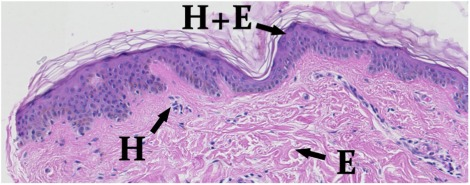
\includegraphics[scale=1.2]{images/HE-stain-example.jpg}
\caption{section of skin showing Hematoxylin(H) \& Eosin(E) stain interactions}
\label{fig:HE-fig}
\end{figure}

\subsection{Slide digitization}
Physical tissue slides are digitized using whole slide image scanners which contain an illumination system, an optical microscope and a focusing apparatus (\textit{\cite{ghaznavi2013digital}}). Scanners most commonly use Brightfield illumination (\textit{\cite{kino1996confocal}}) in which the entire tissue sample is uniformly illuminated. This works in conjunction with the H\&E staining to display the tissue as a dark coloured image on a white background making it easier to distinguish cellular structure. 

The final output of the slide scanner is a virtual rendering of the entire tissue slide, that can be viewed at resolutions of upto 0.25 \si{\micro\meter} corresponding to a 40.0 objective power of the scanning microscope. In order to replicate a slide under a microscope, WSIs exhibit a pyramid structure consisting of images at multiple resolutions. The base level stores the image in diagnostic resolution of a 40.0 objective, often containing 100,000 x 100,000 pixels (\textit{\cite{wang2012managing}}). As displayed in figure(\ref{fig:pyramid-fig}) The resolution is down sampled by a fixed factor at each subsequent level. The Cancer Genome Atlas program's repository contains WSIs with 4 resolution levels down-sampled with factors of 1.0, 4.0, 16.0 and 64.0. This feature of WSIs makes these images extremely bulky with average sizes around 1GB per image. 

\begin{figure}[h]
\centering
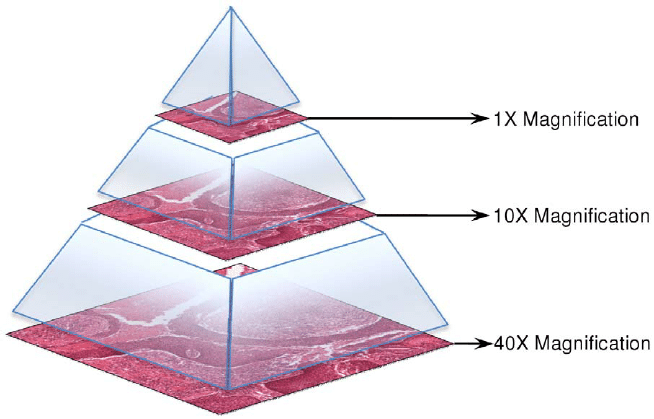
\includegraphics[scale=0.5]{images/digital-slide-stored-in-a-pyramid-structure.png}
\caption{Illustration of pyramid structure observed in whole slide images. Highest resolution at 40.0 magnification followed by 2 downsampled levels at 4.0 (10x) and 40.0 (1x)}
\label{fig:pyramid-fig}
\end{figure}

Viewing or analyzing an entire WSI is infeasible as the whole image simply cannot fit into a standard computer's memory. It was demonstrated by \cite{wang2012managing} that sectioning the WSI into several smaller, fixed size tiles at its diagnostic resolution and performing image analysis tasks on each tile allows for more efficient processing compared to using the entire slide image at once. As shown by \cite{aeffner2019introduction}, confining analysis efforts to smaller regions of interest (ROIs) rather than the entire WSI is often necessary to devise any accurate or computationally viable image analysis algorithms. The tile based results can be aggregated in order to generate masks that highlight all ROIs on lower resolution thumbnails of the original WSI in order to display the results of our image analysis tasks. 

\subsection{Slide normalization} \label{slide-normalization-background}
The manual preparation of tissue slides by pathologists is a very sensitive process and despite having an established staining protocol, several factors can imbue a high degree of variability in the presentation of the resulting WSI. As demonstrated by \cite{anghel2019high}, the lack of consistency in the quality and appearance of slide images is attributed to varying antigen concentration, temperatures at which the tissue is stored, physical conditions the slides are subjected to when being put through slide scanners and random human error involved in the process. \textbf{Figure \ref{fig:he-stain-difference}} illustrates how despite having a standardized staining procedure like the Hematoxylin \& Eosin staining, no two slides of the same tissue will exhibit identical color, stain intensity or physical structure.   

\begin{figure}[h]
\centering
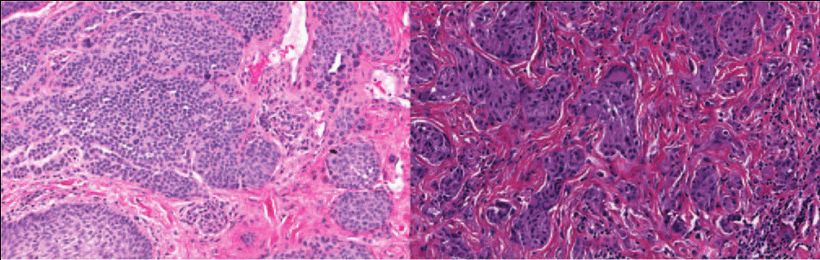
\includegraphics[scale=0.7]{images/stain-difference-slide.png}
\caption{Example of two H\&E stained whole slide images of melanomas obtained from different laboratories indicating the drastic difference in color appearance.}
\label{fig:he-stain-difference}
\end{figure}

\cite{li2015complete} establishes that performing any quantitative analysis on whole slide images requires numerical features obtained from an input image to be compared against features learned from prior training data. The disparities observed between the compared features help quantify any histopathological information conveyed by such images. If there exists additional variability in the WSI stemming from inconsistent slide preparation, then that corrupts the extracted features as they account for these non-histopathological differences and deviate from the true characterization of the sample. There is particularly high colour and intensity variation in slide images sourced from different pathology labs as each location has different conditions and personnel under which slides are produced. According to the paper on automated prostate cancer detection by \cite{gorelick2013prostate}, information conveyed by color variation on tissue samples is of extreme significance in the quantitative analysis of histopathological images. Therefore, it is crucial to achieve greater color consistency by implementing color normalization algorithms when working with models that utilize pattern recognition and color processing algorithms to deliver a diagnosis from learned features. 
\\

\subsection{Macenko method for color normalization}
The Macenko stain normalization method (\cite{macenko2009method}) is considered the gold standard for performing color normalization on H\&E stained whole slide images. This is evidenced by its application in a wide range of works such as, a paper on an end to end learning model for predicting tumour subtypes and genetic mutations from H\&E stained slide images by \cite{van2021deepmed}, predicting colorectal cancer from H\&E stained slides using deep learning by \cite{Kather2019} and \cite{anghel2019high} paper on robust stain normalization system for whole slide images. 

For slide images captured with standard RGB scanners, the stain absorbs three distinct wavelengths of light. \cite{macenko2009method} defines a \textit{stain vector} as the proportion of each wavelength absorbed by the staining component. The overall idea behind this normalization algorithm is that the color of a RGB pixel in a stained slide image is a linear combination of two stain vectors, corresponding to Hematoxylin (H) and Eosin (E). Being able to estimate these stain vectors effectively allows us to project each pixel onto any color plane, thereby converting the WSI into a standardized color profile. The Macenko stain normalization pipeline can be summarized as:
\begin{itemize}
    \item Applying a singular value decomposition (SVD) operation, approximate the H\&E stain vectors of all pixels inside the tissue sample (excluding white background pixels) in a given RGB slide image. 
    \item Apply an intensity correction operation to compensate for irregularities in stain concentration, quality of stain and staining protocol used by the original pathologist. 
    \item Project resulting image on a reference plane to ensure all normalized pixels exhibit a similar color profile. 
\end{itemize}
\hfill\\


\subsubsection{Macenko Algorithm} \label{macenko-alg}
\hfill\\
\cite{macenko2009method} prescribes the SVD based stain normalization algorithm as follows:\\
\\
\textbf{INPUT} : RGB slide image
\begin{itemize}
    \item Transform RGB slide to Opitcal Density (OD) form where \(OD = -\log_{10}(I)\), \(I\) being the RGB vector normalized to \([0.1]\).
    \item Remove pixels with OD intensity less than a pre-determined parameter \(\beta\). \cite{macenko2009method} proved \(\beta = 0.15\) provides the most robust normalization.
    \item Perform singular value decomposition on the OD tuples. Extract the two largest values by magnitude and generate the OD plane in their corresponding direction.
    \item Project input image data onto the resulting OD plane and normalize to unit length.
    \item Calculate \(\theta\), which is the angle of each point with respect to the direction of the \(1^{st}\) SVD value.
    \item Using pre-determined parameter \(\alpha\), calculate robust extremes of the angle which correspond to the \(\alpha^{th}\) and \((100 - \alpha)^{th}\) percentiles. \cite{macenko2009method} empirically recommends a value of \(\alpha = 1\) for the best normalization result. 
    \item Project extreme values back to OD space.
    \item Build optical density matrix (ODM) using the obtained projection from previous step
    \item Inverse ODM to estimate the respective concentration of the Hematoxylin and Eosin stains (\(C_h\) and \(C_e\)). 
    \item Determine the (\(100 - \alpha^{th}\)) percentile of \(C_h\) and \(C_e\).
    \item Upon transforming the normalized concentrations of each individual stain component to OD space, revert it back to RGB using an H\&E reference template. 
\end{itemize}


\begin{figure}[H]
\centering
\begin{tabular}{lccccc}
Raw slide image&
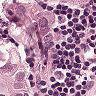
\includegraphics[width=80px]{images/37.jpeg}&
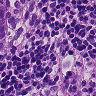
\includegraphics[width=80px]{images/68.jpeg}&
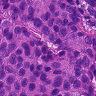
\includegraphics[width=80px]{images/195.jpeg}\\
After Macenko normalization&
 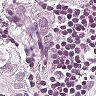
\includegraphics[width=80px]{images/37_macenko.jpeg}&
 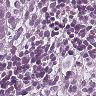
\includegraphics[width=80px]{images/68_macenko.jpeg}&
 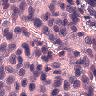
\includegraphics[width=80px]{images/195_macenko.jpeg}\\
 \\&
 (a)&(b)&(c)\\
\end{tabular}
\caption{Examples taken from training data - Illustrating effect of Macenko normalization on WSI patches of varying colour intensities }
\label{fig:macenko-example}
\end{figure}

\section{Deep Learning in histopathological analysis} \label{dl-application-background-section}
\subsection{Applications in WSI based diagnosis} \label{dl-application-background}
As proposed by \cite{gurcan2009histopathological}, diagnosing diseases from histopathological images requires the identification of some histological features, for example, cancer nuclei, glands or lymphocytes that serve as indicators of disease severity. With growing popularity of computer assisted diagnosis systems, Deep Learning has been proven to be the preferred approach for such classification and segmentation tasks on whole slide images. 

\cite{Kather2019} has proposed a supervised learning model that uses transfer learning to train a CNN that performs a patch based classification of nine tissue types observed in H\&E stained whole slide images of Colorectal cancer (CRC) samples. The study used 86 H\&E slides of CRC tissue to create a training set of image patches without any associated clinical data. The CNN was trained on these 224x224 px patches. They were labelled manually with patch-level annotations representing the relevant tissue class. The trained CNN would take a WSI, split it into 224x224 px patches and produce a prediction for the type of tissue a given patch represents with a unique color. Therefore, tile-level predictions were obtained to fully segment the given WSI into its constituent tissues and subsequently extract a deep-stromal score from the multi-class segmented WSI to determine the severity of CRC. 

A paper on detecting invasive ductal carcinoma (IDC) from whole slide images using a CNN was presented by \cite{cruz2014automatic}. As shown in figure \ref{fig:ductal-carcinoma-figure}, the paper proposes a supervised learning model trained using WSI patches containing patch-level annotations to learn a hierarchical  representation of malignant vs benign tissue. The CNN identifies tumour regions to determine tumour extent and severity and subsequently estimate disease prognosis. This deep learning based IDC region classification displayed a 84.23\% accuracy when compared to ground-truth pathologist annotations. The paper presents a comparison of the deep learning approach to more traditional machine learning classifiers implementing a Random Forest method for tumour classification using hand-crafted features like tumour area, texture, nuclear structure, color etc. Using a RGB histogram was only 77.24\% accurate while a fuzzy color histogram showed 78.74\% accuracy, proving the effectiveness of deep learning approaches when performing histopathological analysis. 

\begin{figure}[h]
    \centering
    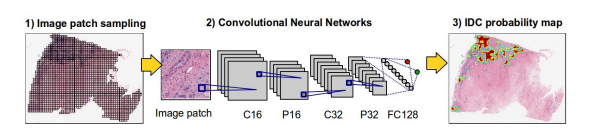
\includegraphics[scale=0.9]{images/Cruz-Roa-Ductal-Carcinoma-example.png}
    \caption{IDC detection framework from H\&E stained WSI - 1)Splitting WSI into tiles, 2)CNN outputs tile-level prediction for probability of being IDC positive, 3)Aggregate predicted tiles to show heatmap of most likely IDC regions with probability > 0.29}
    \label{fig:ductal-carcinoma-figure}
\end{figure}

The use of a patch/tile-based approach to train and segment WSIs is observed to be the most common technique to overcome the memory logistic issues associated with the large size and resolution of WSIs. An alternative approach to processing large WSI data was demonstrated by \cite{qin2018large} using a feature Pyramid method comprising of a ResNet50-GICN-GPP pipeline. The ResNet50 architecture was used as an encoder while combining the feature pyramid blocks as decoders which produced a segemntation accuracy of 63\% when tested on the CAMELYON16 challenge dataset. 

In the context of segmenting malignant breast tissue in H\&E stained WSIs, the paper by \cite{priego2020automatic} proposes a fast semantic segmentation pipeline. As observed in figure \ref{fig:Priego-conv-pipeline}, it performs tile-level segmentation of malignant or benign tissue using a DCNN along with a dilated convolutional encoder-decoder architecture. The paper prescribes using a pre-trained MobileNetV2 network as the backbone of the DCNN. The CNN's max pooling layer is replaced with the convolutional encoder to allow features to be extracted at any resolution, independent of the resolution of the input WSI. This makes it possible to accurately segment regions of the same tissue that may appear different due to scaling disparities in the input image compared to the training images. They applied a softmax function to the last layer of the CNN (as shown in figure \ref{fig:Priego-conv-pipeline}) in order to convert the discrete prediction (malignant vs benign) into tile-level probability maps. These probability maps were merged using a Conditional Random Field (CRF) method that allowed overlapping regions of tiles to be captured more efficiently without any loss of information. 

\begin{figure}[h]
    \centering
    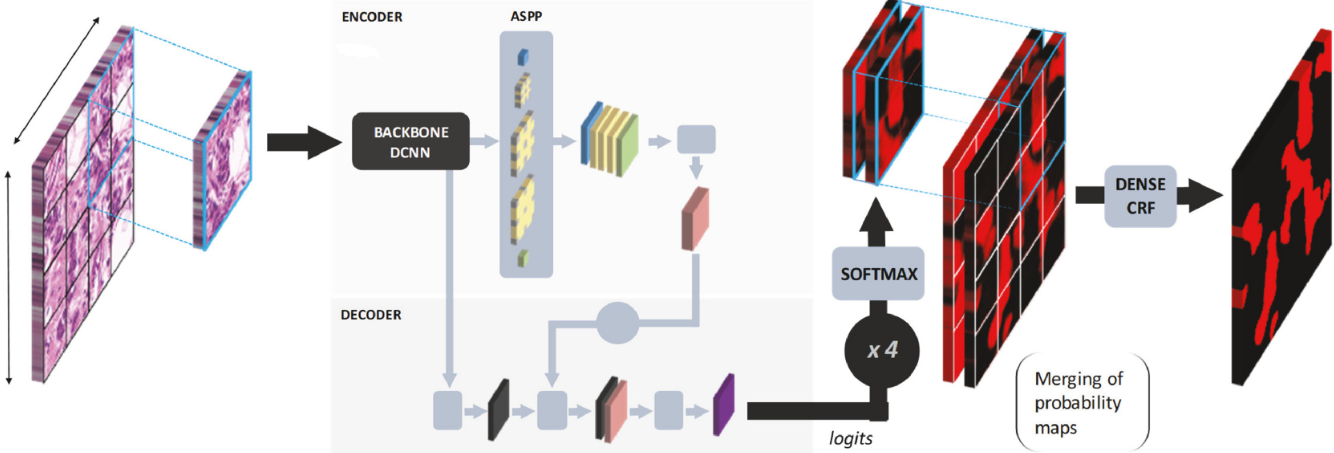
\includegraphics[scale=0.4]{images/Priego-DCNN-encoder-arch.png}
    \caption{\cite{priego2020automatic} - Tile-based semantic segmentation using DCNN and convolutional encoder to obtain probability maps of segmented tissue}
    \label{fig:Priego-conv-pipeline}
\end{figure}

\subsection{Methods to process WSI data for deep learning} \label{background-openslide}
Whole slide images are captured at a minimum 40x magnification resulting in images having resolutions exceeding \(100,000 \times 100,000\) pixels with an average uncompressed size of 5GB (\cite{bandi2018detection}). Thus, a single image often exceeds the available memory size in most computers making it infeasible to perform tasks like patch extraction by loading the entire WSI to memory. This necessitates the use of specialized software to access such images and perform deep learning tasks such as extracting patches for patch-based tissue segmentation.

\cite{bankhead2017qupath} proposes a Java based whole slide processing tool called QuPath. It can be accessed through its own native GUI to perform WSI analysis but also supports Groovy scripts to execute high level algorithms such as patch extraction from WSIs. QuPath also provides the ability to build low level machine learning classifiers like Support Vector Machines or Random Forests within its integrated GUI environment. Recent developments with deep learning are yet to be translated into QuPath as it does not support  training CNNs natively and only allows predictions to be imported and viewed (\cite{pedersen2021fastpathology}). It is also very restrictive due to being a GUI and not having any API support for other languages. The GUI itself has a steep learning curve and is not very intuitive for users who are not experts/researchers in histopathology. 

\cite{goode2013openslide} have created Open Slide which is an open-source, vendor-neutral C library for viewing, processing and analyzing WSIs. The major problem in digital pathology is the lack of a standardized format for WSI. This causes WSI vendors to create their own proprietary format that requires their proprietary software to process. Open Slide aims to increase interoperability by facilitating transparent handling of various vendor formats of WSIs while supporting multiple programming language APIs. It offers a Python package to enable WSI processing through Python which makes it accessible for academic research.   

\subsection{Data availability for CNN training} \label{data-availability-section}
As reported in the paper on Colorectal Cancer diagnosis from histology slides by \cite{Kather2019}, all data used in training and validation of the CNN was manually annotated by an expert pathologist. They sectioned 86 CRC H\&E whole slides from the NCT biobank and UMM pathology archive to create a training set of 100,000 tiles. Each tile had to be manually annotated at a tile level. to describe the nine relevant tissue classes. Their validation set comprised of 862 H\&E slides retrieved from 500 CRC patients on The Cancer Genome Atlas (TCGA) repository. Data from TCGA does not contain any pixel or slide level annotations and had to be manually reviewed to identify relevant histological artifacts. 

\cite{priego2020automatic} further lay emphasis on the lack of publicly available H\&E stained whole slide images with strong pixel level annotations being a major hindrance in the development of supervised learning models. Their solution to this lack of annotated data was to create an OpenSlide based, online WSI viewer that allowed pathologists from across the world to view and hand annotate tumour regions, thereby constructing a training dataset tailored to this project for breast cancer lesion segmentation.

The CAMELYON16 and CAMELYON17 challenges were identified as viable data sources for training deep learning models to detect breast cancer metastases. \cite{Khened2021} proposed a generalized framework for WSI segmentation and validated its performance in breast cancer segmentation using CAMELYON16 and CAMELYON17 data. As shown by \cite{bejnordi2017diagnostic} in their paper on deep learning algorithms for breast metastases detection, the CAMELYON16 data serves as a very robust dataset for training supervised learning models as it contains 399 WSI (159 malignant and 240 benign samples), sourced from two separate laboratories with pixel level annotations of breast metastases found in sentinel lymph nodes. 

CAMELYON17 on the other hand was showcased by \cite{bandi2018detection} in assessing potential deep learning techniques for breast cancer detection and prognosis assessment. This dataset was built upon CAMELYON16 to include 1399 WSI of breast metastases in sentinel lymph node sections, sourced from five different laboratories to more accurately represent staining variability and allow for more robust training. Instead of pixel level annotations, CAMELYON17 included slide level annotations to allow for a shift of focus on patient-level diagnosis followed by patient prognosis prediction rather than diagnosing metastases in individual WSI. 
\\
\subsubsection{Why is CAMELYON data effective for diagnosing breast cancer?}
\hfill\\
The effectiveness of CAMELYON16 and CAMELYON17 data in diagnosing breast cancer despite containing lymph node biopsies is explained by \cite{sobin2011tnm} in their TNM staging system. In diagnosing breast cancer, clinicians consider the extent of tumour growth (T-stage), spreading of tumour cells to lymph nodes (N-stage) and the degree of metastases in other parts of the body (M-stage). Presence of breast metastatic cells in sentinel lymph nodes, which is the first lymph node breast cancer cells drain into, is therefore a significant indicator of breast cancer prognosis and can be used to learn how to characterize general breast metastases in deep learning models.


\section{Cancer prognosis estimation}
\subsection{Survival time analysis methods} \label{survival-analysis-methods}
As an extension to deep learning based CRC diagnosis, \cite{Kather2019} have proposed fitting a uni-variable Cox-proportional Hazard model with features extracted from each tissue class to model their respective influence on patient-level survival prediction. Utilizing a Youden index \((sensitivity + specificity - 1)\), they determined an optimal Hazard Ratio (HR) cutoff value. All counts of tissue classes with HR > cutoff were weighted with their HR and combined to develop a deep stromal score quantifying slide-level disease severity. They propose a further step to fit a multivariate Cox proportional hazard model on the TCGA validation data, in order to adjust for clinical factors like tumour stage, sex and age when obtaining the Hazard Ratio. This multivariate HR showed higher confidence in prognosis predictions as it accounted for both slide-level tissue morphology and patient specific clinical factors. 

Other instances of survival analysis on histopathology images, such as the paper by \cite{Wetstein2022} illustrates a Kaplan-Meier survival analysis using a uni-variable and a multivariate Cox proportional hazard model. The multivariate analysis was included to produce more realistic survival predictions that accounted for clinical characteristics of each patient, such as current treatment, tumour dimensions and lymphovascular state. All these factors are ignored by the uni-variable model which only aims to utilize histological features in its prediction. A similar methodology was also proposed by \cite{Liu2022} using univariable Cox proportional hazard models. They having additionally demonstrated the use of Python's \textit{Lifelines} package in streamlining the Cox model fitting process and KM plot generation to visualize survival events. 

Majority of work in the field of automated survival estimation involves linear parametric Cox models as described previously. The applicability 
of these methods are constrained by the requirement of strong, pixel-level annotations in facilitating supervised learning models to extract precise features to successfully quantify survival. Alternate approaches of survival analysis are still being developed but are not as prominently established.  \cite{katzman2018deepsurv} proposed a feed-forward neural network called DeepSurv to quantify the influence of a patient's clinical and histological covariates on their hazard rate and subsequently support treatment recommendations. This method uses an alternate approach to  previously described linear Cox regression by using a neural network to optimize the partial likelihood loss function of the Cox model using non-linear features. \cite{wulczyn2020deep} illustrates another method of survival prediction using a weakly supervised learning approach. Uniformly sampled patches were drawn from the slides of a given patient, only knowing if the slide was malignant or benign. Image-based features extracted by the CNN from these patches were processed by a custom loss function - combination of cross-entropy and Cox partial likelihood loss - to output a probability distribution over discretized survival intervals for each patient.

\subsection{Cox proportional hazard model} \label{cph-background}
The original paper by \cite{cox1972regression}, demonstrated a generalized regression method as an extension to the Kaplan-Meier survival analysis approach. The Cox proportional hazard model is a linear regression model defined in terms of a hazard function (\(\lambda\)) as follows
\begin{equation}
    \centering
    \lambda (t | \textbf{x}) = \lambda_0 (t) \exp (\beta \textbf{x})
    \label{eq:hazard model}
\end{equation}

where \(t\) represents time, \textbf{\(x\)} denotes an \(n \times 1\) element vector of all covariates being modelled such that \(n=1\) for univariable Cox modelling and \(n > 1\) for multivariable models. \(\beta\) represents a vector of all regression coefficients in the model while \(\lambda_0 (t)\) denotes the baseline hazard under initial conditions of \(\textbf{x} = 0\). 

This hazard model displays the relation between the time until some event occurs (in survival models the event is the death of a subject) to the given covariates. The proportional nature of the model implies a multiplicative increase in hazard rate with unit increase in the covariate(s). This can be demonstrated by considering a univariable model where \(x\) and \(\beta\) are both one element vectors representing single covariate regression. Following a unit increase in the covariate, such that we have \(x + 1\) as our new covariate, the new hazard function is
\begin{equation}
    \centering
    \begin{aligned}
        \lambda (t | x + 1) ={}& \lambda_0 (t) \exp (\beta (x+1)) \\
                            ={}& \lambda_0 (t) \exp (x\beta  + \beta)) \\
                            ={}& (\lambda_0 (t) \exp (x\beta)) + \exp (\beta) \\
                            ={}& \lambda (t | x ) \exp (\beta)
    \end{aligned}
\end{equation}

denoting a constant multiplicative scaling by \(\exp (\beta)\) of our original hazard function upon a unit increase in covariate. Furthermore, upon changing sides of the new hazard function we get
\begin{equation}
    \centering
    \begin{aligned}
        \frac{\lambda (t | x + 1)}{\lambda (t | x )} = \exp (\beta) 
    \end{aligned}
\end{equation}

where the ratio \(\exp (\beta)\) is a constant with no time dependence. This represents the "proportional" nature of the Cox hazard model where the relationship over time between original and subsequent hazard functions remains constant despite changing covariates. 

\subsection{Kaplan-Meier analysis} \label{km-background}
The Cox proportional hazard model only describes the hazard or probability of certain survival event happening at a specific point of time. It is useful in analyzing the risk of survival associated with given features. However, it cannot predict overall survival time as hazard is inversely proportional to survival, with survival showing rapid decline at high hazard function values. As defined by \cite{bewick2004statistics}, having survived until a given time \(t\), the hazard function \(\lambda (t)\) corresponds to the probability of dying at \(t\). Whereas, the KM survival function \(S(t)\), represents probability of surviving until time \(t\). \cite{schober2021kaplan} proposes using the Kaplan-Meier method for producing exact survival time predictions. Kaplan-Meier generates a parametric survival function that estimates the probability of patient surviving past a certain point of time. Showing overall survival time prediction using Kaplan-Meier graphs is the most common methodology as observed in all survival analysis papers such as \cite{Kather2019}, \cite{Liu2022} and \cite{Wetstein2022}.

\begin{figure}[h]
    \centering
    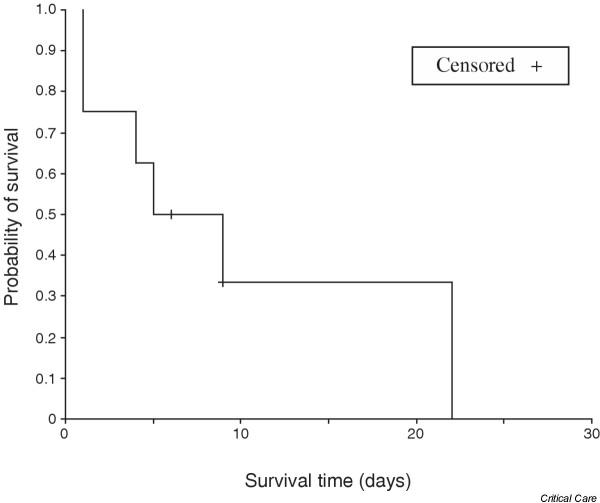
\includegraphics[scale=0.3]{images/KM-plot-example.jpg}
    \caption{\cite{bewick2004statistics} - Example Kaplan-Meier plot showing overall survival probability }
    \label{fig:km-plot-example}
\end{figure}

As observed in figure \ref{fig:km-plot-example}, a KM plot is a step-wise function plotting probability of survival on the y-axis and survival time in any discrete unit on the x-axis. KM plots can support multiple curves on the graph where each represent a unique covariate setting to see their influence on survival. The graph displays vertical drops in survival probability over time at points where an event of interest occurs, which in survival analysis is the death of a subject. The horizontal distance to these points on the curve represent the total interval of time after which the event occurred, thereby showing the probability a subject survives for that period of time. As proposed by \cite{bewick2004statistics}, the median survival time is often a good prediction of overall survival as it is the point of 0.5 probability where half the subjects perish and the other half lives. This median survival time can be used to compare multiple KM plots in terms of how severely  covariate influences survival.  

%==================================================================================================================================
\chapter{Analysis}
\section{General Problem}
\subsection{Cancer detection} \label{cancer-general-problem}
The first step to delivering a cancer prognosis from histopathological images is to quantify disease severity and extent through image-based features. As illustrated in figure \ref{fig:camelyon16-example}, there is a clear visual difference between malignant and healthy tissue samples. Firstly we observe in figure \ref{fig:camelyon16-example} - (b), that tumour cells are enclosed within distinct patches among the non-background pixels rather than being homogeneously dispersed throughout the body of the tissue. Secondly in figure (c) we observe a difference in stain intensity between the surrounding healthy cells and the tumour within the annotation lines. This color disparity is caused by abnormal cellular growth - displaying an increase in the size of Hematoxylin stained (blue) nuclei and reduced nuclei density leading to an increase in Eosin stained (pink) cytoplasm observed in tumour regions. 

\begin{figure}[H]
\centering
\begin{tabular}{lccccc}
Normal tissue&
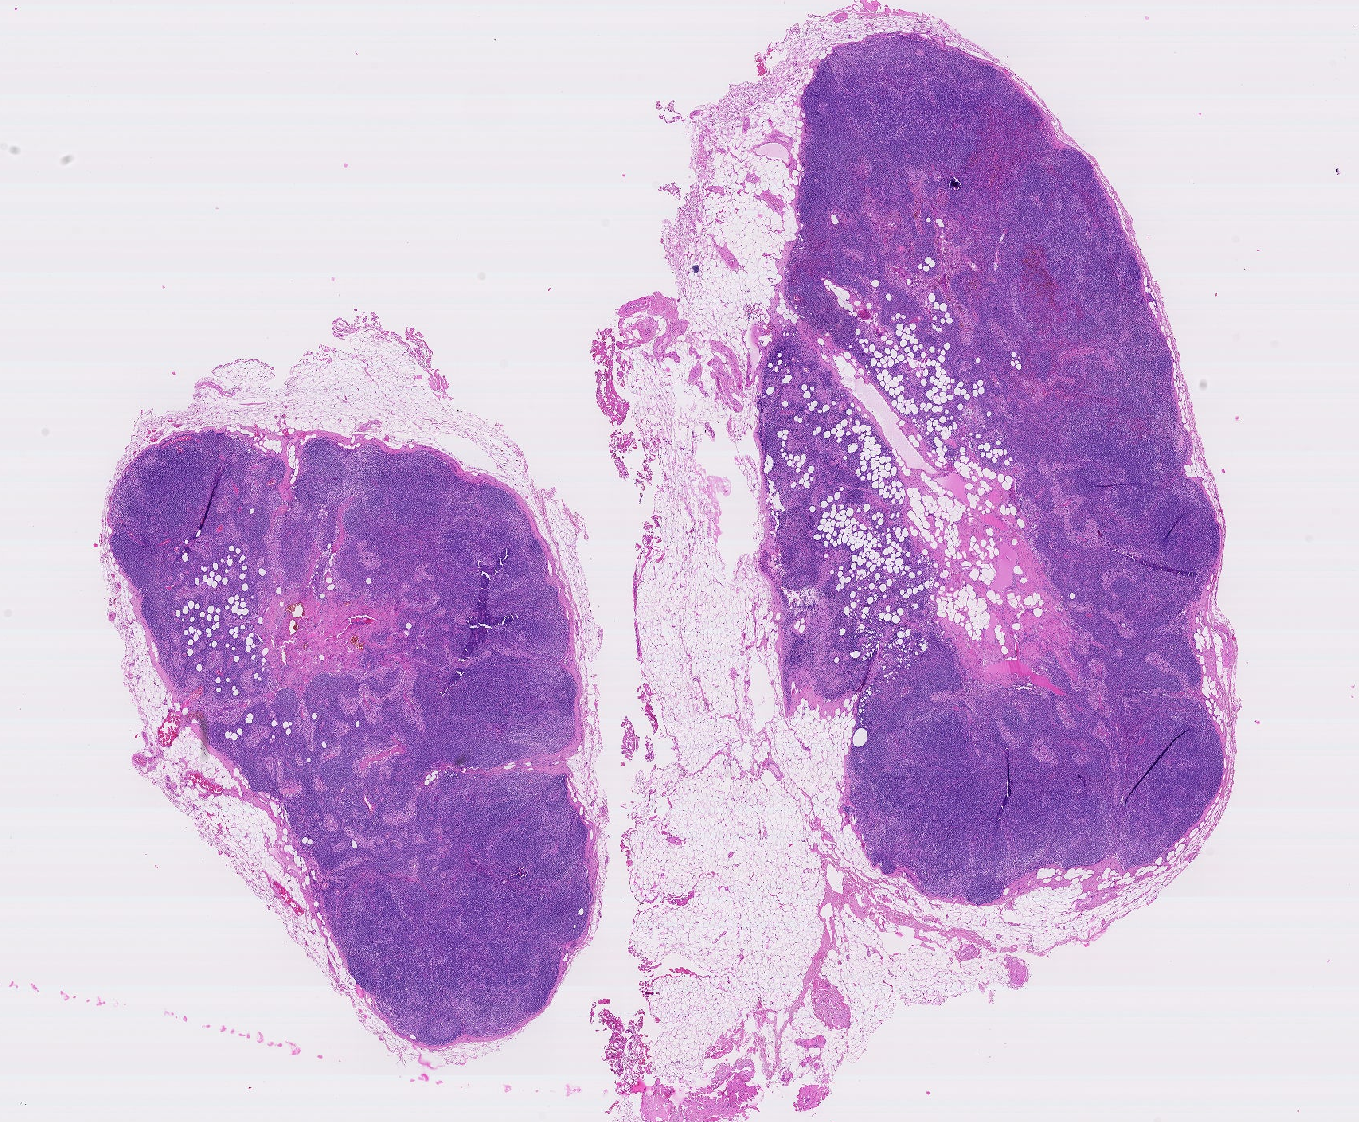
\includegraphics[width=100px]{images/camelyon16-normal-example.png}&
\\&
(a)\\
Malignant tissue&
 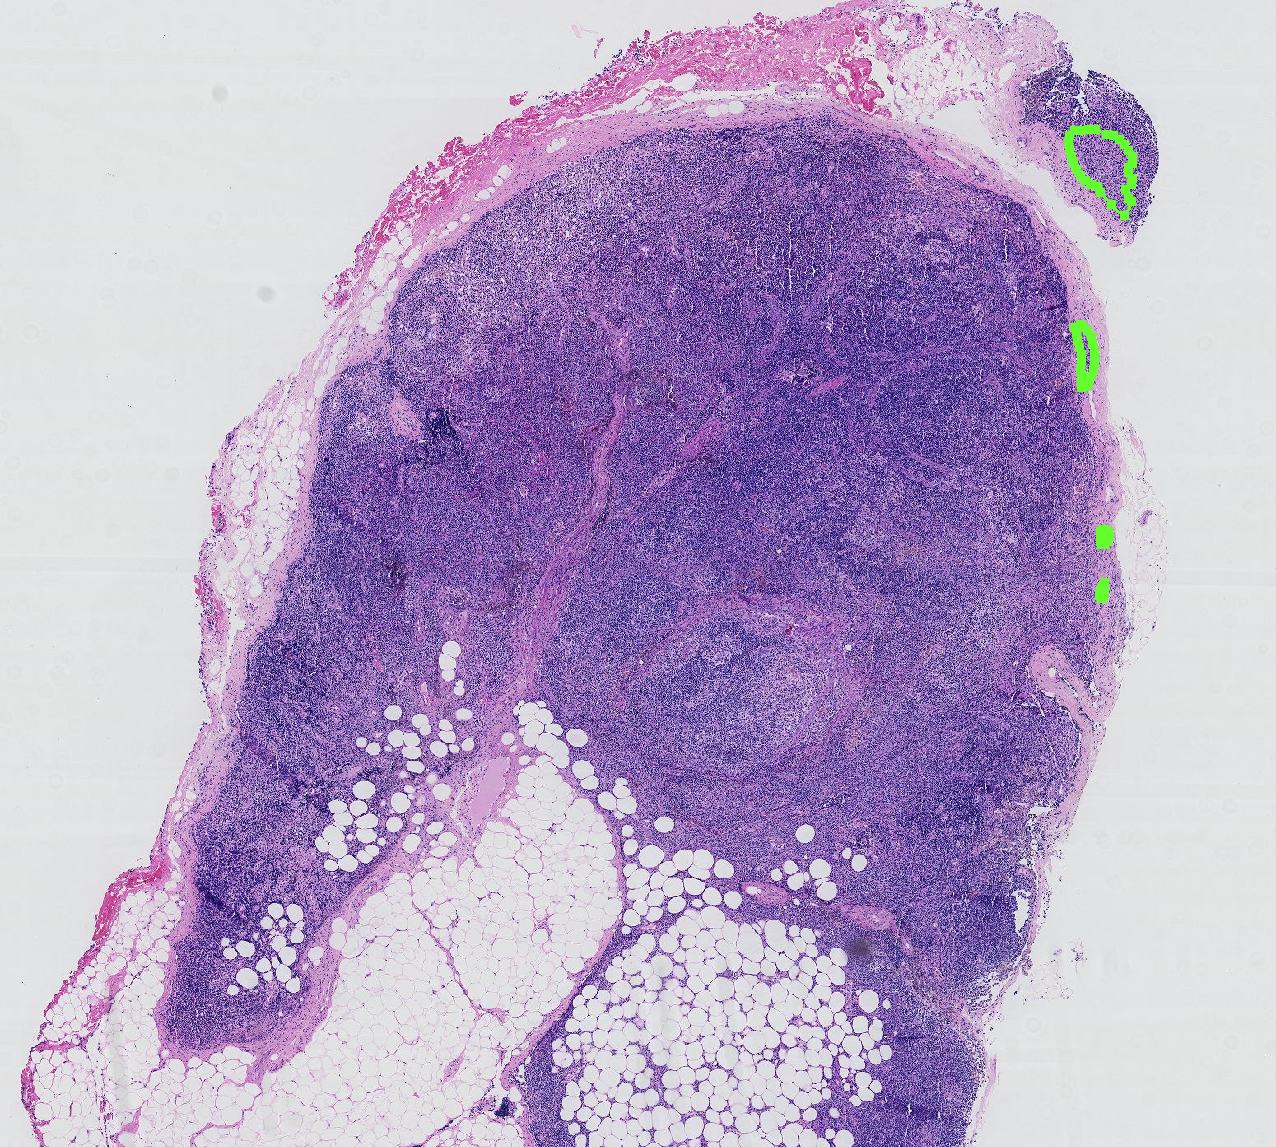
\includegraphics[width=100px]{images/Camelyon16-cancer-example1.png}&
 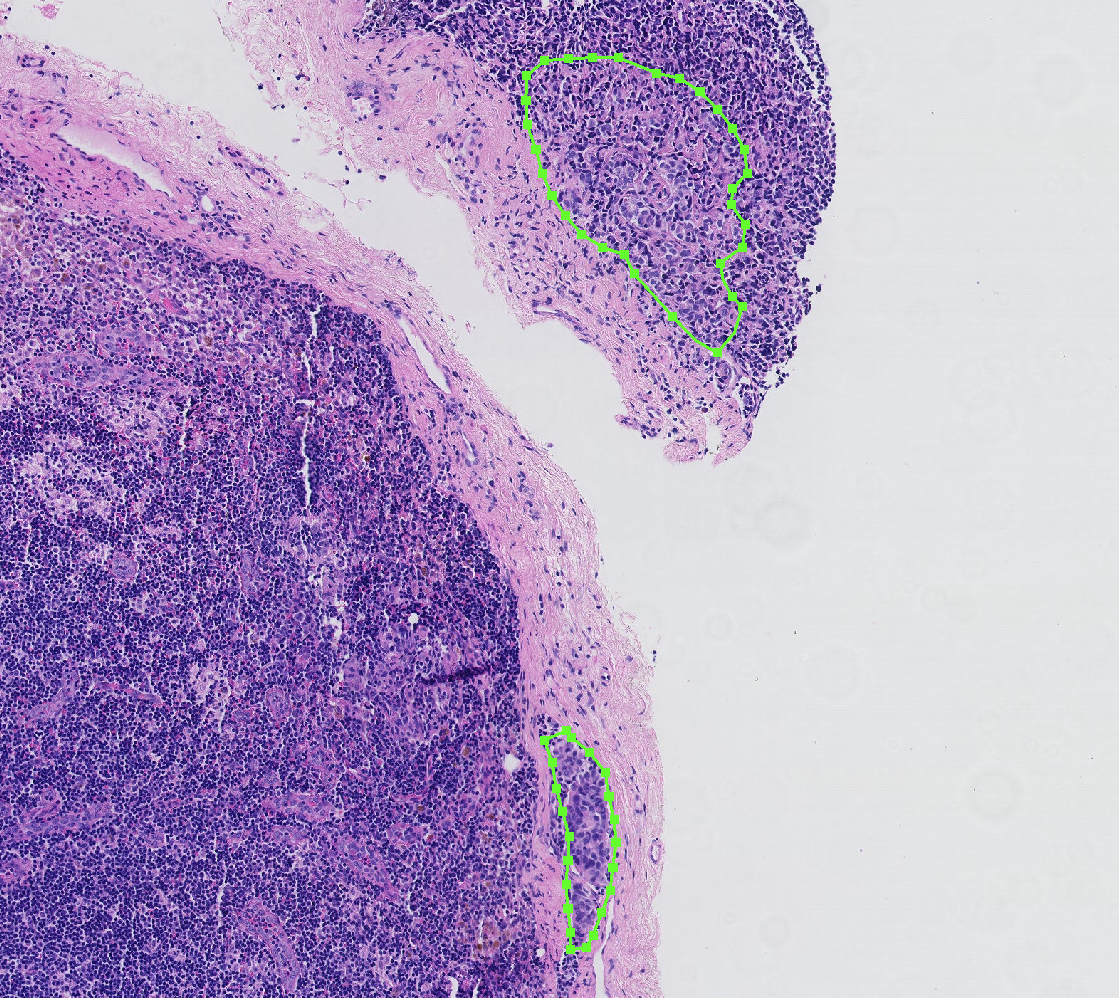
\includegraphics[width=100px]{images/Camelyon16-cancer-example2.png}&
 \\&
 (b)&(c)\\
\end{tabular}
\caption{Examples taken from CAMELYON16 training data - Normal tissue (a) exhibits healthy breast tissue with no cancerous tumour. Malignant tissue (b) represents annotated location of malignant tumour with respect to the overall slide and (c) displays a closer view of malignant cells inside annotated region}
\label{fig:camelyon16-example}
\end{figure}

The general problem we are trying to solve at this stage is to identify whether a given tissue slide is cancerous and subsequently segment its malignant areas to extract meaningful features that convey disease severity and extent. As prescribed in multiple literature reviewed in section \ref{dl-application-background} we can perform a tile-based analysis of the whole slide image. Using the visual differences observed in healthy and cancerous cells, we can predict tiles as malignant or benign based on their constituent cellular morphology. Tumour areas will be detected by high density of tiles predicted as malignant and thereby segmenting the WSI into regions of interest. Since we know a given WSI has a fixed pixel count at the sampling resolution, we can quantify the extent of a tumour in terms of the pixel area covered by malignant tiles. As inferred from figure (\ref{fig:camelyon16-example}), the difference in stain intensity of tumour cells compared to healthy cells can be used to quantify cancer severity in terms of an aggregated color intensity metric of malignant tile regions. Severely abnormal nuclear growth in tumour regions will produce much darker stain intensities due to large nuclei, whereas severe cytoplasmic expansion will display significantly lighter color intensities compared to healthy cellular regions.

\subsection{Survival time estimation}
As explained by the literature reviewed in section \ref{survival-analysis-methods} we can utilize the image-based features extracted from the previous stage as covariates to fit Cox proportional hazard models. This will allow us to obtain the hazard function for each feature and measure its influence as a risk factor affecting survival of patients. The CPH models for each covariate enables comparison between different features to identify their relative significance in prognosis estimation. The final problem of predicting the overall survival time can then be solved by generating Kaplan-Meier plots of the most significant covariates and obtaining the median survival time from the graph as shown in figure \ref{fig:km-plot-example}. These fitted models can be generalized to any WSI given as input, by first processing the WSI as tiles through our CNN to extract the relevant features. These features are mapped to our fitted regression models to genearte its corresponding KM plot and deliver the final disease prognosis in terms of a median survival time. 

\section{Whole slide images}
\subsection{Data availability}
As discussed in section \ref{data-availability-section}, the most widely used approach for automated cancer detection from histopathological images requires large datasets with strong, pixel-level annotations to train a robust supervised learning model. Creating our own custom dataset to train and validate our model would involve sourcing sufficiently diverse WSIs and having an expert pathologist manually annotate over 100,000 tissue patches for our tile-based approach, which extremely resource intesive and infeasible for the scope of this project. Therefore, this paper uses CAMELYON16 data as our training dataset since it has been annotated at a pixel level by expert pathologists.

\subsection{PCAM dataset for model training} \label{pcam-background}
We have utilized the PatchCAMELYON (PCAM) version (\cite{Veeling2018-qh}) which is a pre-tiled, publicly available dataset containing over 327,000 tiles sourced from 399 WSIs included in the CAMELYON16 data. The PCAM data comprises of 96x96px tiles with binary tile-level annotations indicating whether a tile is malignant or benign based on the presence of cancer cells in the center 32x32px patch of each tile. The CAMELYON16 WSIs are provided a 40.0 objective but PCAM tiles are undersampled by 10x to increase field of view. The PCAM dataset replicates the same train/test split thresholds as the CAMELYON16 dataset, including 50/50 balance between malignant and benign tiles with no overlap to allow unbiased model training. PCAM also holds out 20\% of training tiles to create a validation set to allow models to be cross validated. The tile annotations are provided as CSV files in the following format:

\begin{center}
\begin{tabular}{ |c|c|c|c|c|c| } 
 \hline
 id & coord\_y & coord\_x & tumor\_patch & center\_tumor\_patch & wsi \\ 
 \hline
 1 & 148544 & 74048 & 1 & 1 & camelyon16\_train\_tumor\_003 \\ 
 \hline
\end{tabular}
\end{center}

The X and Y coordinates represent the pixel coordinate of the top-left vertex of the 96x96px tile taken from the whole slide image specified in the wsi column. A binary (0 or 1) annotation is provided for each tile. A value of 1 for tumor\_patch indicates the presence of cancer cells located anywhere within the 96x96px tile. Whereas, an annotation of 1 for center\_tumor\_patch indicates that malignant tissue is present in the center 32x32px patch of the tile. 

\section{Processing}
\subsection{Supervised learning and survival prediction}
After reviewing the methods employed by other research papers in section \ref{dl-application-background-section}, we will be utilizing a supervised learning model to solve the first stage of our general problem. This model will employ a tile-based approach to learn how to segment WSIs into malignant and benign regions. We will employ the strongly annotated PCAM data as the training dataset for our CNN. This will be an end-to-end learning model that learns how to characterize malignant and benign tissue and output a fully segmented representation of the input WSI with clearly demarcated tumour regions. The segmented image will then be used to extract features that can meaningfully quantify disease severity in a given histopathological sample. 

For the second stage of our general problem, we aim to develop a model that can produce overall survival time predictions based on certain quantifiable features extracted from a given WSI by our trained CNN. To arrive at a generalizable survival model we will need to curate a model training dataset containing these image-based features along with clinical labels of associated survival time prognosis for each WSI. Based on our previous discussion in section \ref{data-availability-section}, TCGA data has been proven to be a credible and high-quality data source for clinically relevant histopathological images. Another advantage of TCGA is that each sample also includes diagnostic data, such as the survival time predicted by pathologists for each patient's case. We will apply our trained CNN to a collection of breast cancer WSIs sourced from TCGA to extract image-based features. These features will be used as covariates along with associated survival time  labels to fit linear Cox regression models and Kaplan Meier plots that can be generalized for overall survial time predictions.

\subsection{Image pre-processing}
The PCAM dataset used to train our CNN to solve the first stage of our general problem is a derivative of the CAMELYON16 database, which is a vast and diverse collection of histopathological samples sourced from multiple pathology laboratories. As discussed in section \ref{slide-normalization-background}, variability in preparation conditions introduces inconsistencies to the quality and appearance of WSIs. This makes it necessary to apply Macenko normalization to our PCAM data before using it to train our model. This ensures that our model learns to characterize the true morphological difference between malignant and benign breast tissue samples rather than learning the random noise introduced in the appearance of the WSI during preparation.

When applying this model to TCGA breast cancer slides to extract image-based features, we must split the WSI into tiles and eliminate background dominant tiles. Furthermore, we perform Macenko normalization on each tile to make our input data  consistent relative to our model's trained features and ensure accurate segmentation of malignant regions. 

\subsection{Ground truth validation}
For the purpose of training a deep learning model to detect breast cancer we require histopathological data with clinically valid labels to actually learn how to characterize the morphology of breast metastases. The CAMLEYON16 dataset has been manually annotated by expert pathologists and will serve as the basis of training for our cancer detection model. We will then optimize the trained model hyperparameters and measure its performance in segmenting malignant regions of histopathological images against the annotated validation set of the PCAM data. 

As described previously, the second stage of our problem aims to develop a regression model that can be generalized to predict an overall survival prognosis given breast cancer biopsy images as input. Fitting this model requires pathologically valid labels of associated survival time predictions of each WSI used in populating the relevant feature dataset. These ground truth labels for each WSI sourced from TCGA can be accessed through cBioPortal, which is a large scale genomic dataset containing the accompanying diagnostic data for each histopathological sample image hosted on TCGA. The performance of the fitted survival model will then be measured on unseen WSI samples taken from TCGA and the corresponding survival prediction will be validated against available diagnostic data on cBioPortal. 

%==================================================================================================================================
\chapter{Design}
\section{Cancer detection system overview} \label{sec:detection-overview-design}
We implement a neural network to solve the first stage of our overall problem. Figure \ref{fig:sys-overview} illustrates a logical workflow of how we go from an input breast tissue slide to a segmented malignancy feature map. As seen in the upper half of the figure, the network is first trained with batches of WSIs, each sectioned into labelled, colour-normalized tiles. During the training process, every RGB tile will undergo a series of convolutions as it passes through each layer of our network. Neurons will learn a weight based on the feature representation extracted by kernel convolutions in each layer. The final layer's output is thresholded to give a class prediction for the tile. This is compared to ground truth label and a loss is calculated. Our goal if to minimize this loss value. This is achieved by using an optimizer to backpropagate and update the weights of each neuron to improve the learned feature representation and produce more precise predictions. 

\begin{figure}[h]
    \centering
    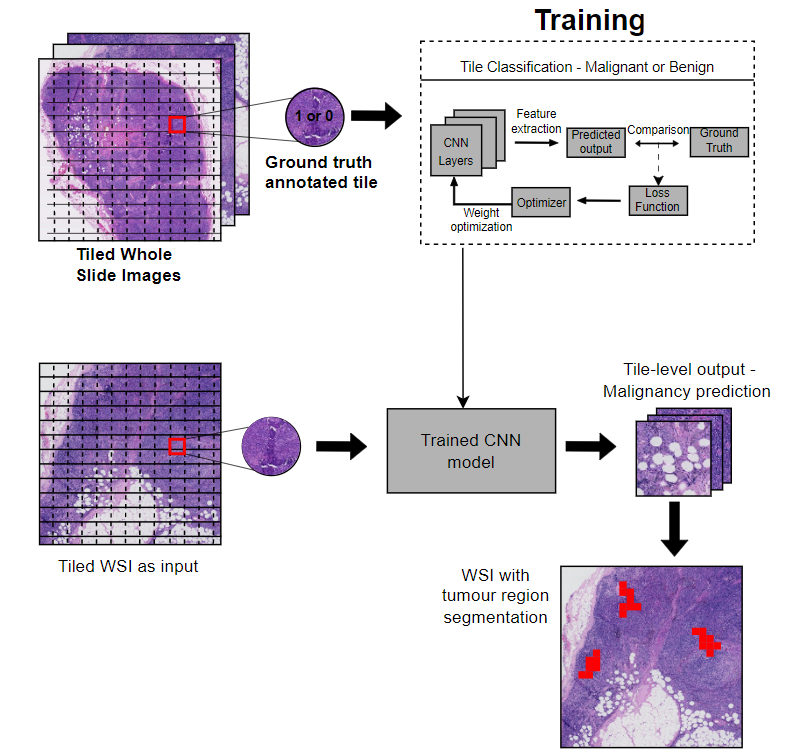
\includegraphics[scale=0.7]{images/system-overview-1.png}
    \caption{Workflow of cancer detection system design. The upper half of the figure demonstrates the training procedure of the neural network. It uses annotated WSI tiles to learn feature representations of breast metastatic tissue samples. The training will use the ground-truth annotations of each tile to optimize the neuron weights and minimize training loss. In the lower half of the image, the trained model is used to produce tile-level, binary predictions for a given WSI. The predicted tiles, marked as malignant or benign, are used to generate a segmented feature map of the original WSI}
    \label{fig:sys-overview}
\end{figure}

 The trained model will process an input WSI on a tile-by-tile basis to estimate the presence of cancer cells in each tile. Using the learned feature representations of breast cancer morphology, the neural network performs a binary classification task to output the most likely class (malignant (1) or benign (0)) for each tile. The tiled predictions will be overlaid on a thumbnail of the WSI to produce a segmented feature map indicating potential tumour regions, as illustrated in figure \ref{fig:sys-overview}. We repeat this process for a series of WSIs taken from the TCGA repository to generate a collection of segmented feature maps. For the next stage of our problem, we will manipulate this feature dataset to extract covariates that can effectively model and estimate survival time. 

\subsection{Tiling and pre-processing} \label{tiling-design}
Since the CAMLEYON16 data is sourced from multiple pathological laboratories, we will be applying the Macenko normalization alogrithm (section \ref{macenko-alg}) on each tile of the PCAM dataset before training our model. This normalization will allow the model to learn features of cellular morphology in tiles, based on their actual structure rather than accounting for differences in colour appearance and treating them as different features. This introduces colour invariance to allow the model to more accurately identify similar tissue artifacts across different WSIs. 

The WSIs processed by our CNN to generate segmented tumour maps for the survival analysis, must be tiled individually as TCGA only contains whole histopathological slides. To maintain consistency between training and feature extraction tiles, there are two main points to consider - tile dimension and tile resolution. We utilize the OpenSlide library described in section \ref{background-openslide} to convert a WSI into a stream of tile objects of specified dimension at a chosen resolution level. Therefore, we extract \(96 \times 96\)px tiles sampled by 10x to a 4.0 objective to match the PCAM tile dimensions.

Figure \ref{fig:undersample-example} illustrates that a tile sampled at 4.0 magnification (10x undersample) shows a much wider field of view compared to a 40.0 objective tile. As explained in section \ref{cancer-general-problem}, detecting tumour regions is based on identifying abnormally large nucleus or increased cytoplasm dispersion. The lower resolution exposes spatial information that allows our model to identify regions of abnormal nuclear growth relative to surrounding cellular structure. The 40.0 magnification however, zooms in on individual nuclei to the point where any information on spatial locality is lost and our model cannot characterize nucleus size or distribution. 

\begin{figure}[H]
\centering
\begin{tabular}{cc}
 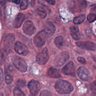
\includegraphics[width=80px]{images/45_117.png}&
 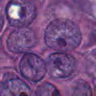
\includegraphics[width=80px]{images/119_239.png}\\
 (a)&(b)\\
\end{tabular}
\caption{Illustrates two tiled sections sampled from a TCGA WSI, used in feature dataset generation - (a) \(96\times96\)px tile sampled at 4.0 objective shows greater field of view and less granular detail (b) \(96\times96\)px tile sampled at 40.0 objective has smaller field of view and shows individual nuclei at greater detail}
\label{fig:undersample-example}
\end{figure}

All tiles obtained will be Macenko normalized in order to allow for colour invariant predictions from our model. We must also remove any blank tiles that are predominantly background. This reduces the computation time of our cancer detection pipeline by only processing tiles containing relevant tissue artifacts. The tile filtering will be done by choosing an intensity threshold representing the average intensity of Macenko normalized H\&E stain and eliminating all tiles with higher average intensity. 

\subsection{Tumour prediction - classification and segmentation} \label{sec:classication-design}
Tiling is equivalent to dividing a given image into a grid of \(96 \times 96\)px squares. Each tile extracted from a WSI will be stored in disk along with an X-Y coordinate representing its location on the grid. We will generate two types predictions from the CNN - a discrete binary class prediction and a continuous prediction of the likelihood of being malignant. The results from the CNN will be stored against each tile's coordinate in a dataset format. This dataset will serve as the feature dataset for survival analysis. 

In order to visualize the tumour segmentation, we first generate a thumbnail of the WSI downsampled to a resolution that allows viewing the entire image without causing memory issues. For the binary prediction, we map a distinct colour to each of the two classes. For each tile, we overlay the associated colour to its corresponding coordinate on the thumbnail. This creates a sharp segmentation between normal and potential tumour regions of the tissue. Using the continuous predictions, we can generate a complete heatmap showing the exact likelihood of regions being malignant on the tissue surface. The predictions will be a probability value between 0 and 1, which we map to a continuous colour scale thresholded to the same range and overlay the associated colour on each tile coordinate. 

\section{Survival estimation - regression}
\subsection{Model covariates} \label{sec:covariates}
\subsubsection{Malignancy spread score} 
\hfill\\
Using the binary predictions obtained from our cancer detection model, we develop a scoring system to quantify the extent of malignancy in a given WSI. We estimate the degree of tumour spread in terms of pixel area covered by malignant tiles. This is equivalent to the number of tiles assigned a malignant 
class (=1) prediction by our CNN. Not all WSIs are the same size, with some including multiple or much larger tissue sections which would naturally consist of a higher number of non-background tiles. To prevent this metric from showing disproportionately high tumour spread for larger WSIs, we normalize the malignant tile count by the total area covered by non-background tiles. This produces a ratio representing the size of metastatic tumours as a percentage of overall tissue surface in a WSI. The score can then be used as a covariate that quantifies cancer severity in modelling overall survival time prognoses. 

\subsubsection{Mean malignant intensity}
\hfill\\
The continuous predictions generated by our model are in the form of a probability value between 0 and 1 showing the likelihood of a given tissue patch being malignant. This represents the confidence  associated with each prediction that can be inferred as intensity of malignancy. A high probability corresponds to a tile with strong malignant features that are distinctly identifiable. Whereas, low probability indicates weakly malignant or benign morphology observed in the tile. We calculate the mean malignant intensity of a WSI by taking the average probability across all its tiles. A high mean intensity score (closer to 1) will translate into a more severe metastatic characterization caused by the presence of dominant regions of strong malignant predictions. A lower mean intensity (closer to 0), will correspond to majority low probability tiles (benign if <0.5) indicative of less severe metastasis. 

\subsection{Survival time prediction}
\subsubsection{Regression training data}
\hfill\\
In order to fit a generalized model that can estimate overall survival time for a given breast cancer slide, we first build a model training dataset. This will be developed using a collection of 75 WSIs sourced from TCGA. We restrict the WSI selection process to deceased patients with available diagnostic data only. For each WSI, we retrieve the ground truth label of the patient's actual survival time (in months) - the duration from point of diagnosis to point of death - available on cBioPortal against the patient's TCGA case ID. Using survival times of \textit{deceased} patients as the basis of our model allows us to estimate an upper bound of how long patients survive with different levels of cancer severity. Every WSI will be processed through our trained CNN to generate segmented tumour maps. The severity of each WSI will then be quantified by extracting the feature metrics described in the previous section. The final dataset will consist of an overall survival duration and a value for the covariates against each WSI to fit the regression model. \\

\subsubsection{Survival model}
\hfill\\
As described in section \ref{cph-background}, we fit a Cox proportional hazard model using the training dataset described above to generate hazard functions for each covariate. This allows us to determine each feature's significance and validity as a risk factor impacting survival time of patients. As described in section \ref{km-background}, we then predict the median survival time estimate from Kaplan Meier plots generated by querying our model with the associated coavriate levels of the given WSI. 

The final pipeline to obtain a survival time estimate for a WSI is as follows:
\begin{itemize}
    \item Section WSI into 96x96px tiles at a 4.0 objective
    \item Macenko normalize each tile
    \item Generate tile level malignancy predictions using trained CNN 
    \item Calculate Mean Malignant Intensity and Malignancy Spread Score for the WSI
    \item Query fitted survival model to generate KM plots for each covariate level  
    \item Compute the median survival time from the fitted model
\end{itemize}

%==================================================================================================================================
\chapter{Implementation}
\section{System overview}
We have implemented a separate system corresponding to each of the two main stages of breast cancer analysis - diagnosis and prognosis. The diagnostic system generates both continuous and discrete predictions of malignant regions present in a breast tissue WSI. This system is trained using clinically annotated breast cancer slides as ground truth labels. The resulting predictions are used to extract features that quantify disease severity in terms of metastatic spread. Finally, the prognostic system fits a regression model using the diagnostic features to predict an overall survival time for each patient. We essentially perform 4 distinct high-level tasks: training, diagnostic predictions, model fitting and survival predictions. 

\subsection{Training overview}
Due to the extremely resource intensive process of strongly annotating cancer WSI tiles by hand, we have used the PCAM dataset for training our neural network to perform cancer detection. The dataset contains tiled breast metastases WSIs sourced from the CAMELYON16 database along with associated tile-level binary annotations indicating if a tile is malignant (1) or benign(0), which is used as the ground truth labels.

We have implemented a pre-processing pipeline (as shown in figure \ref{fig:implementation-overview}),  to prepare any input data into a format that can be processed by our neural network. We first feed our training data through this pipeline, skipping the tiling step as the PCAM dataset is already tiled into \(96 \times 96\)px patches. We subsequently normalize the colour of each tile using the Macenko algorithm to allow our model to achieve colour invariant. In the final stage of pre-processing we perform data augmentation to synthetically expand our training space with random variants of each tile, allowing our model to be more robust by learning rotational and translational invariance.

\subsection{Malignancy predictions overview}
As discussed in section \ref{sec:detection-overview-design}, we have curated our own feature extraction dataset consisting of 75 WSIs sourced from TCGA. Using our trained neural network, we perform a tile-based binary classification task on each WSI to generate fully segmented feature maps indicating potential tumour regions. This implies that each WSI will be fed through the pre-processing pipeline (as shown in figure \ref{fig:implementation-overview}), without the data augmentation step, to generate colour normalized tiles which our trained model will then generate predictions for. The final predictions will be used to extract a malignancy spread score and mean malignant intensity as described in section \ref{sec:covariates}.

\begin{figure}[H]
    \centering
    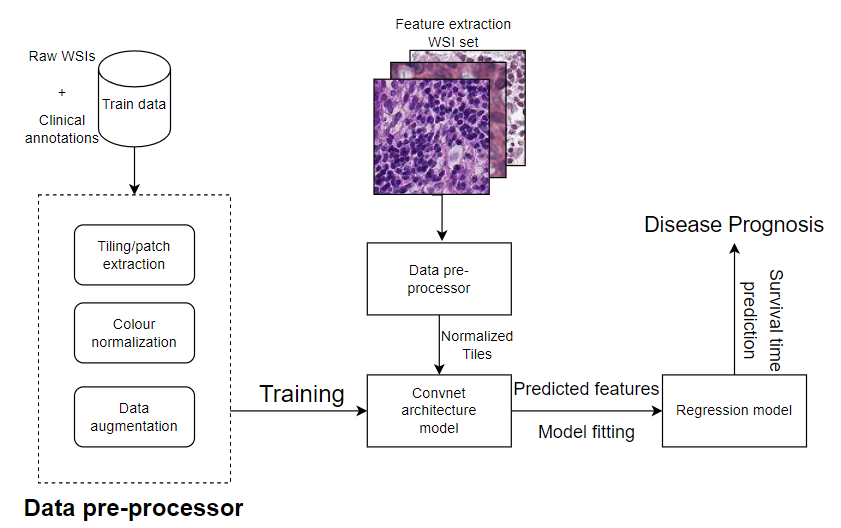
\includegraphics[scale=0.7]{images/implementation-overview.png}
    \caption{Complete overview of our entire system implementation. PCAM data containing raw WSI tiles and ground truth annotations are used as training data. The tiled dataset is colour normalized and augmented using our pre-processing pipeline before being used to train our convnet architecture based neural network. We curate a feature extraction dataset containing WSIs from TCGA. Each WSI is pre-processed into colour normalized tiles and fed through our trained model to generate feature maps indicating malignant regions. Predicted features are then used to fit a parametric Cox regression model which uses Kaplan-Meier method to generate a median survival time prediction.}
    \label{fig:implementation-overview}
\end{figure}

\subsection{Survival time predictions overview}
Our neural network will generate discrete and continuous predictions that will be used to extract two scores that characterize the disease severity in terms of tumour spread of the given WSI. For all 75 WSIs in our feature extraction dataset, we also obtain their clinically determined survival times to serve as ground truth labels for our survival model. Finally, we use the predicted scores along with survival time annotations to fit a parametric Cox regression models for each metric. Each model generates a hazard ratio and a negative log-likelihood indicating the associated risk factor of the covariate and the significance of impact on survival respectively. We then produce a median survival time estimate from the models to compare their performance with respect to the corresponding ground truth survival time and evaluate their effectiveness in survival prognosis estimation.

\section{Machine Learning - Cancer diagnosis}
\subsection{Datasets}
\subsubsection{Training data}\hfill\\
For the purpose of training our neural network model to make breast cancer predictions, we have utilized the tiled and annotated version of the CAMELYON16 challenge data called the Patch CAMELYON (PCAM) dataset. It contains 399 WSIs, tiled into over 300,000 total tiles. Each tile is annotated with a binary annotation indicating malignancy nature as described in section \ref{pcam-background}. Tiles are \(96 \times 96\)px in dimension with their resolution undersampled by 10x to a 4.0 objective rather than the 40.0 native objective. 

The PCAM data contains separate datasets for training, validation and testing, each with an equal balance between malignant positive and healthy (malignant negative) tiles. Each set is stored in a Hierarchical Data Format version 5 (HDF5) file. This format stores extremely large (in this case 200,000 images) data in a structured format resembling an entire file system hierarchy as a single file. It allows individual data points to be accessed in an efficient manner without needing to transfer entire datasets to memory and as a result overloading available memory. 

In an HDF5 file data is organized into groups representing folders. These groups contain other groups or the datasets which resemble files. As seen in listing \ref{lst:pcam-hdf5}, each PCAM dataset contains two main groups labeled 'x' and 'y' under the root. The 'x' group holds the WSI tiles, represented as \(96 \times 96 \times 3\) numpy arrays of 8bit unsigned integers (0 to 255) under groups labled with a unique id for each tile. The 'y' group holds the malignancy annotation of each tile. The annotation is a binary label that is stored under the group with id corresponding to the tile it labels. 

\begin{lstlisting}[language=python, caption={PCAM Data HDF5 schema - Each set has a group labeled 'x' - containing all the tiles as numpy arrays of 8-bit unsigned integers. Each array has a unique id (0, 1, 2...) and shape \(96 \times 96 \times 3\) indicating a \(96 \times 96\)px RGB tile. The second group labeled 'y' contains the annotations for each tile. The annotations are shown as binary labels against each tile id. }, label= lst:pcam-hdf5]
    # root group
    /
        # image data group
        x/
            # tile id group
            0/
                [96 x 96 x 3 - 8bit unsigned integer numpy array]
            1/
            2/
            ...
        # annotation group
        y/
            # tile id group
            0/
                0
            1/
                1
            2/
            3/
            ...
\end{lstlisting}

We iterate over the HDF5 datasets and save the numpy array of each tile as a \texttt{.jpeg} image into a \texttt{/tiles} directory within each of the three dataset directories. We extract 100,000 training tiles and 20,000 validation tiles, both equally balanced between the two classes, for example, the training tiles consist of 49,977 malignant (1) and 50,023 benign (0) tiles. We also extract the corresponding annotations from HDF5 format into a \texttt{.csv} file, indexed by the tile id as described in section \ref{pcam-background}. This allows for more efficient data handling through the CNN using dataloader objects that can readily associate batch of images to their corresponding labels during the training process. 

\subsubsection{Feature extraction data}\hfill\\
We also created a second dataset consisting of raw WSIs to serve as the basis of extracting malignancy features required to develop a survival model for making survival time predictions. This dataset consisted of 75 WSIs sourced from the TCGA breast cancer repository. We cross checked each WSI's TCGA ID against the clinical data on cBioPortal to only select WSIs which had associated clinical data available showing overall survival time and belonged to deceased patients. This allowed us to retrieve the overall survival duration for each patient, given the malignancy condition displayed by their biopsy sample to serve as ground truth labels for our survival model. All TCGA WSIs have a native 40.0 magnification at the highest resolution level and an average file size of 2GB due to their large pixel count. Images were downloaded and stored in disk in a \texttt{.svs} format which supports multi-level resolution sampling.  

\subsection{Data pre-processing}
We store all relevant data in their raw format before being used with our machine learning model. As explained previously, histopathological slide images are subject to high levels of irregularities caused by conditions under which they were produced. Furthermore, WSIs are extremely massive images, which in their raw format simply cannot be processed in an online fashion like standard machine learning problems. Therefore, we have developed a general pre-processing pipeline consisting of  operations that convert the raw image data into a consistent format that can be processed more efficiently by our neural network. This pipeline performs three main operations - tiling, colour normalization and data augmentation. 
\\
\subsubsection{WSI Tiling}\hfill\\
The PCAM training data consists of pre-tiled WSIs with each tile having dimensions \(96 \times 96\)px and a 10x downsampled resolution. As explained in section \ref{tiling-design}, we have to ensure we tile each WSI in the feature extraction dataset using the same dimensions so that our model can make meaningful predictions based on the model weights learned from PCAM tiles. We utilize the OpenSlide package to tile the WSIs without needing to load the entire image into memory. 

We fetch each WSI's \texttt{.svs} file from disk and open it as an \texttt{open\_slide} object as shown in listing \ref{lst:tiling-code}. This allows us to inspect the slide's metadata using \texttt{slide.properties} attribute and choose which level number corresponding to our desired sampling resolution. We then use the \texttt{DeepZoomGenerator} object which takes as parameter the WSI as an \texttt{open\_slide} object, the tiling dimension and an overlap percentage to convert the slide image into a stream of tile references. 

\begin{lstlisting}[language=python, caption={Code excerpt showing how OpenSlide and DeepZoomGenerator are used to obtain tiles of specified dimension and resolution level from an input WSI image and saming them as a .tiff image. We also added a modification to normalize each tile (explained in the next section) before saving. It calls \texttt{macenko\_norm\_HnE()} on each tile's numpy array and saves the normalized image. We also catch any SVD convergence errors thrown by tiles that have large areas of white space. This is the case for external tiles containing debris outside the main body of tissue.}, label= lst:tiling-code]
    from openslide import open_slide
    from openslide.deepzoom import DeepZoomGenerator
    slide = open_slide(wsi_file_path)
    tiles = DeepZoomGenerator(slide, tile_size=96, overlap=0, limit_bounds=False)
    level_num = (tiles.level_count)-2
    cols, rows = tiles.level_tiles[level_num]
    for row in range(rows):
            for col in range(cols):
                temp_tile = np.array(tiles.get_tile(level_num, (col, row)).convert('RGB'))
                if temp_tile.std() > 15 and temp_tile.mean() < 230 and temp_tile.shape == (96,96,3):
                    try:
                        macenko_norm, h_norm, e_norm = macenko_norm_HnE(temp_tile)
                        tiff.imsave(save_path, macenko_norm)
                    except np.linalg.LinAlgError as LinAlgError:
                        tiff.imsave(save_path, temp_tile_RGB_np)
\end{lstlisting}

We set the desired resolution level - it is the 2nd highest level for TCGA WSIs that exhibit a 10x downsampling to 4.0 objective. We iterate over each tile reference and obtain the individual tile image as a Numpy array at the specified resolution. We must also filter out any tile that is majority blank background in order to reduce our overall processing space and prevent unnecessary computation. We completely tiled a sample WSI to analyze a collection of its tiles. On average undesirable tiles with majority white background had a mean pixel intensity of >230. Whereas, useful tiles with significant tissue content had an average pixel std deviation of >15. Therefore, a mean intensity lower than 230 indicates the presence of darker tissue regions on the tile. Furthermore, a std deviation of greater than 15 indicates greater variance in pixel intensity values, implying that the darker regions are significant enough for the tile to not be majority white space. As shown in the above code, we filtered out all tiles that did not meet the mean and std deviation requirements before saving each tile as a \texttt{.tiff} file.
\\

\subsubsection{Macenko normalization}\hfill\\
As described in section \ref{slide-normalization-background}, we follow the standard algorithm prescribed by Macenko to implement a function that accepts as input a tile image and returns a colour normalized tile. 

We implemented a \texttt{macenko\_norm\_H\&E()} function that takes as parameters the input image and  normalization factors. We use the recommended parameter values of \(\alpha = 1\) and \(\beta = 0.15\). Additionally we also provide a normalizing factor of \(IO = 240\), taken from the MATLAB implementation \footnote{https://github.com/mitkovetta/staining-normalization} of the algorithm. Our implementation calculates the optical density (OD) of our input image and eliminates transparent pixels below the \(\beta\) threshold. We perform an SVD operation using \texttt{np.linalg.eigh} on the OD matrix and project it onto the plane represented by the largest eigenvalues using a dot product with the corresponding eigenvectors. Computing the angles in the direction of the first SVD we find its robust extremes. These angles determine the individual stain vectors corresponding to Hematoxylin and Eosin components. Using the obtained HE matrix, we determine the least square solution to the equation \texttt{HE @ X = Y} using \texttt{np.linalg.lstsq(HE, Y)} where Y represents the OD matrix of the input image. The computed solution is the concentration factor that scales the HE matrix to obtain the given image's stain appearance. We finally normalize the obtained concentration by dividing it using maximum H\& concentration values and recreate the input image in the normalized colour space. This is finally projected back to RGB space and returned as the final Macenko normalized image along with the H-image and E-image as shown in figure \ref{fig:macenko-code-example}.

\begin{figure}[h] 
    \centering
    \begin{subfigure}[b]{0.2\textwidth}
        \includegraphics[width=\textwidth]{images/35.jpeg}
        \caption{Default tile}
        \label{fig:default-tile}
    \end{subfigure}
    ~
    \begin{subfigure}[b]{0.2\textwidth}
        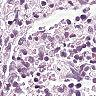
\includegraphics[width=\textwidth]{images/mnorm.jpeg}
        \caption{Normalized Tile}
        \label{fig:mnorm-tile}
    \end{subfigure}
    ~ %add desired spacing between images, e. g. ~, \quad, \qquad, \hfill etc. 
      %(or a blank line to force the subfigure onto a new line)
    \begin{subfigure}[b]{0.2\textwidth}
        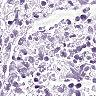
\includegraphics[width=\textwidth]{images/h.jpeg}
        \caption{H-component tile}
        \label{fig:h-tile}
    \end{subfigure}
    ~ %add desired spacing between images, e. g. ~, \quad, \qquad, \hfill etc. 
    %(or a blank line to force the subfigure onto a new line)   
    \begin{subfigure}[b]{0.2\textwidth}
        
\includegraphics[width=\textwidth]{images/e.jpeg}
        \caption{E-component tile}
        \label{fig:e-tile}
    \end{subfigure}
    \caption{Illustrating effect of Macenko normalization on the base H\&E stained tile. Additionally shows the H-component tile with prominently highlighted nuclei and the E-component highlighting cytoplasmic distribution}
    \label{fig:macenko-code-example}
\end{figure}

 As shown in listing \ref{lst:tiling-code}, we extended the tiling pipeline by applying a normalization function on each tile's Numpy array and saving the normalized version. There is code to catch any convergence errors thrown by Numpy's \texttt{linalg.eigh} function that is often quite unstable and can fail when values are too high. This is the case with external and tissue edge tiles that contain large areas of white background but pass our mean intensity filter due to having high std deviation caused by presence of debris. 



\subsubsection{Data augmentation}\hfill\\
Following good scientific practice when working with limited training data, we have implemented a series of data augmentation steps as a method of synthetically expanding our training data space by including randomized variations of existing images. We utilize \textit{torchvision.transforms.Compose()} to combine a series of random translational transforms, each with occurrence probability of p = 0.5, and a single 45 degree random rotational transform. The final step is a \texttt{.ToTensor()} transform that converts the image variant into a format that the CNN can readily process. The custom dataset class (explained further in section \ref{training-implementation}) applies these data transformations to each image that is fetched from the dataset during the model training loop. Data augmentation also serves to give our model rotational and translational invariance allowing it to make more robust predictions irrespective of the image orientation. 

\subsection{Neural network architecture} \label{cnn-architecture}
Following the most common approach to solving image analysis tasks using deep learning model, we have implemented a convolutional neural network based on the state-of-the-art ConvNet architecture. Our implementation utilizes a series of standard convolution layers followed by dense layers to produce the final class prediction. We have implemented our CNN using the PyTorch \footnote{https://pytorch.org/} library for Python. 

As illustrated in figure \ref{fig:CNN-Arch-diagram}, we provide tensors of RGB tiles having dimension \(96 \times 96 \times 3\) as input to our CNN. The input is received as image batches which we have set to a batch size of 32. Next, the images are passed through 4 hidden convolution layers, each using a \(3 \times 3\) kernel with default values for padding = 0 and stride = 1. The first layer convolves the (3, 96, 96) shaped image tensor using 8 total filters to produce an output of dimension (8, 94, 94). At every subsequent hidden layer, the number of filters is increased by a factor of 2 (8 \(\rightarrow\) 16 \(\rightarrow\) 32 \(\rightarrow\) 64) which in turn progressively doubles the channel dimension while reducing the image size. The output from each hidden layer is passed to a Max Pooling layer with a kernel size and stride of 2. This downsamples the image dimensions exactly by a factor of 2. Max Pooling allows the neurons to retain the weights of the most prominent features from the convolved feature map which allows the model to identify any abnormalities in cellular morphology that can indicate malignancy. We also apply a \(\tanh\) activation function to all hidden layers. After 4 layers of convolutions, pooling and activation, the output feature maps has dimension (64, 4, 4) which is then passed to the classification layers. 
\\

\subsubsection{Classification unit}\hfill\\
The fully convolved batch of \(4 \times 4 \times 64\) feature maps are each flattened into a 1D tensor of dimensions \(1 \times 1024\) and then fed to the classification unit composed of 2 fully connected layers. Only the first layer is given a \(\tanh\) activation. We tried using a ReLU activation for the hidden layers and the first fully connected layer, which is the most standard activation function used nowadays. However, a ReLU activation produced outputs that were all biased towards a single class so we chose the \(\tanh\) activation instead. We then apply a dropout layer with  probability of 0.75 over the default value of 0.5. This is a regularisation step aimed to reduce over-fitting by randomly dropping a fraction of the neuron connections from the previous layer. This introduces noise to the training process and forces the current layer to be more robust by making predictions from sparse input. The  output from the second FC layer represents a 2 element tensor and consists of the respective feature weights for the two prediction classes. Since our model uses a negative log likelihood loss function during training, we applied a log\_softmax activation to obtain the final output of our model as log probability of the two relevant classes. 

\begin{figure}[h]
    \centering
    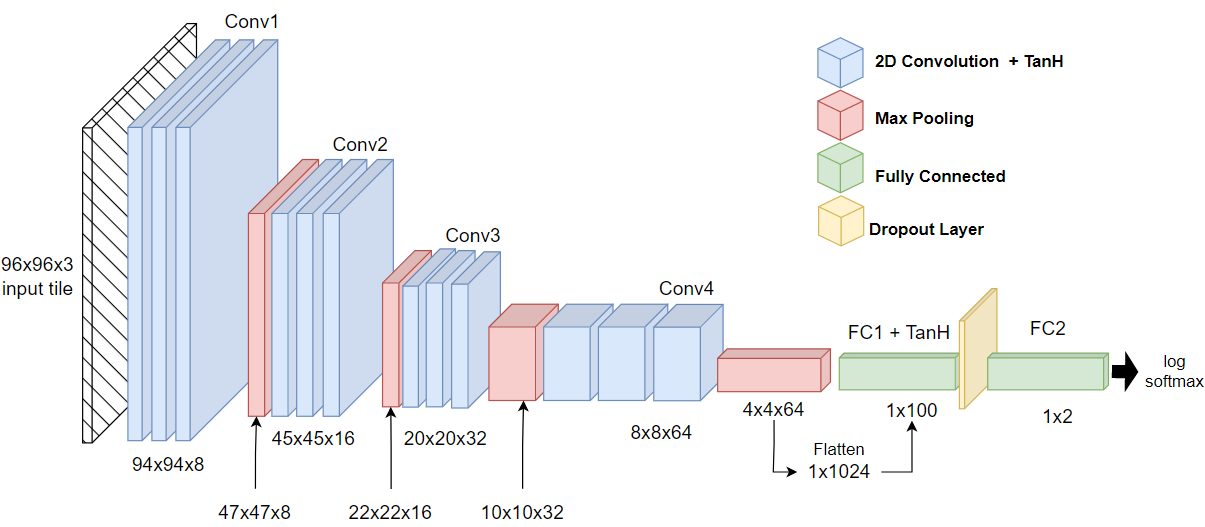
\includegraphics[scale=0.5]{images/CNN-arch.png}
    \caption{Our implemented model follows a standard ConvNet architecture for image classification. The first part of the network involves 4 \(\times\) 2D convolution layers with a TanH activation on each hidden layer. The convolution layers use a 3x3 kernel with padding=0 and stride=1. Starting with 8 filters in the first layer, they increase by a factor of 2 in each layer. Each hidden layer is connected to a Max Pooling layer that extracts the most prominent feature from the previously generated feature map. Each pooling layer, using a 2x2 kernel with stride=2, compresses the previous convolution layer's output map by a factor of 2. The final pooling layer's output is flattened into a 1x1024 element tensor which is used to generate binary class predictions by 2 fully connected layers. The first FC layer has a TanH activation which feeds into a dropout layer with p=0.2. This drops 20\% of random connections from the previous layers at every iteration to make the model more robust and avoid overfitting. The final FC layer's output is log-softmaxed to obtain log probabilities corresponding to the two prediction classes.}
    \label{fig:CNN-Arch-diagram}
\end{figure}
 

\subsection{Training} \label{training-implementation}
\subsubsection{Data loading}\hfill\\
The HDF5 format is usually very memory efficient when dealing with large datsets allowing us to load relevant slices of data into memory. However, we are required to perform pre-processing tasks on individual images and then feed the resulting images through the neural network. It was highly memory inefficient to extract images from the HDF5 dataset, pre-process them and then hold all images in memory for further processing. Therefore, we read raw images from the disk, feed them through the pre-processing described above and write processed images back to disk. Listing \ref{lst:dataset-class}, displays the solution we implemented for continuous and efficient data fetching from disk for model training. We utilize a dedicated dataset component, to fetch processed images from disk and create a stream of image references and their labels which we pass to PyTorch dataloaders to seamlessly extract image batches and feed them to our CNN for training and validation. 

\begin{lstlisting}[ language=python, caption={Custom \texttt{breastCancerDataset} class to fetch all training and validation images and ground truth labels from a given base directory. It creates objects associating each image's path in disk with its corresponding label to make a stream of data that pytorch's dataloaders can readily use to fetch batches of images without needing to initially load all images to memory}, label= lst:dataset-class]
    class breastCancerDataset(Dataset):
    def __init__(self, data_dir, transform, data_type='train'):
        # path to images
        data_path = os.path.join(data_dir, data_type+"/tiles")
        # get list of images
        fnames = os.listdir(data_path)
        self.full_fnames = [os.path.join(data_path, f) for f in fnames]
        # labels are in a csv file names train_labels.csv
        labels_path = os.path.join(data_dir, data_type+"/" + data_type + "_labels.csv")
        labels_df = pd.read_csv(labels_path)
        # set data frame index to id
        labels_df.set_index("id", inplace=True)
        # obtain labels from data frame
        self.labels = [labels_df.loc[int(f[:-5])].values[3] for f in fnames]
        self.transform = transform
    def __getitem__(self, index):
        if isinstance(index, slice):
            start = 0 if index.start == None else index.start
            stop = -1 if index.stop == None else index.stop
            step = 1 if index.step == None else index.step
            images = []
            for idx in range(start, stop, step):
                img = Image.open(self.full_fnames[idx])
                img = self.transform(img)
                images.append(img)
            return images, self.labels[start:stop:step]
        else:
            # open image, apply transform and return with label
            image = Image.open(self.full_fnames[index])
            image = self.transform(image)
            return image, self.labels[index]
\end{lstlisting}

\subsubsection{Model training and validation}
As explained previously, we used the PCAM dataset's training data consisting of 100,000 histological tiles to train our model to detect malignant tissue. The training set was balanced with equal distribution between the two predictable classes. The PCAM dataset also provides a dedicated validation set which we limited to 25,000 images to use for model validation during training. 

We create PyTorch dataloaders for each dataset by fetching images from disk using our custom dataset class. We process training data in batches of 64 images. As explained previously, we use random transformations on training data to augment the dataset. However, we don't use data augmentation on the validation set and only transform each validation image into a PyTorch tensor. To train our model, using a \textbf{Negative Log Likelihood} loss function was appropriate because we have a single-label, binary class classification problem. The model also uses an \textbf{Adam} optimizer with an initial learning rate of 0.0005. This was chosen over the standard SGD method because SGD has a single, fixed learning rate for all weights. Adam maintains separate learning rates for each neuron weight that get updated independently as learning unfolds allowing for more robust feature learning. Consequently, we use a \textbf{ReduceLROnPlateau} learning rate scheduler which allows the model's learning rate to be reduced whenever learning stagnates in an attempt to improve model learning. During training process, we simultaneously calculate NLLLoss for both training and validation batches. While training loss is used to backpropagate and update neuron weights using our optimizer, the validation loss is used with the LR scheduler to reduce the model's learning rate by a factor of 0.5 if the loss does not show any improvement for 20 consecutive epochs. 
\\
\subsubsection{Training time}\hfill\\
Our CNN model was trained using pytorch's CUDA package to take advantage of GPU accelerated processing, thereby reducing training time significantly. The model was trained on a system with current state-of-the-art NVIDIA RTX 3070 GPU. The training time for our model was a bottleneck as we are required to train on 100,000 images and validate against 25,000 images every epoch and we used 100 epochs for our model training. This total training time ranged between 2 to 5 hours based on our batch sizes.
The prediction stage using our trained model proved to be even more significant as a computational bottleneck. Generating tumour maps of 75 WSIs involved predicting over 2 million tiles and processing 800GB of total image data through our model. The entire feature dataset took over 8 hours to be generated each time making repeated feature extractions infeasible.
\\
\subsubsection{Hyperparameter tuning}\hfill\\ \label{impl-hyperparam}
We have undertaken a parameter space exploration task to identify the most optimal configuration for our model, particularly the activation function, learning rate, batch size and dropout rate. We have utilized PyTorch's \texttt{Ray[Tune]} package to automatically search through combinations of parameter settings and find the most optimal configuration. We avoided exhaustively testing every possible combination of parameter values as that was causing a "combinatorial explosion", crashing the entire process due to overloaded GPU memory. Therefore, we chose to test 20 models with randomly sampled parameter values from the given search space. Using each model's validation loss as the chosen performance metric, we have identified the most optimal configuration  for our final model that we illustrated in section \ref{cnn-architecture}. Given the scale of training and validation data we used, each tuning model took around 8 to 10 minutes to complete every training epoch which added up to over 13 hours for a single model to be trained and evaluated over 100 epochs. Thus, we trained our parameter tuning prototype models on a 10,000 image subset of our training data (still maintaining a 50-50 class balance). We also reduced the training epochs to 50 as that was sufficient to get a general idea of which parameter settings were trending in the optimal direction. Furthermore, \texttt{Ray[Tune]} allows setting a \texttt{grace\_period=10} parameter to the tuning process which automatically stops training and discards a model if it does not show improvement in performance metrics for over 10 epochs.
 

\section{Regression - Survival time prediction}
\subsection{Feature extraction and visualization}
As explained previously we have curated a dataset of 75 breast cancer WSIs from TCGA to extract relevant features characterizing their malignancy severity and build a survival time model around those features. We feed each WSI through our pre-processor and subsequently generate a prediction for each individual tile. All predictions for a single WSI are stored in a \texttt{.csv} file as labels against  grid coordinates of its tiles - binary predictions display a 0 or 1 label and continuous predictions display a probability value of belonging to class 1 (malignant). We have then used the \texttt{Pandas} library to process this structured prediction data and calculate, for each WSI, its Malignancy Spread Score and Mean Malignant Intensity as explained in section \ref{sec:covariates}. 

As shown in figure \ref{fig:visualization-example}, we also implemented a visualization pipeline using \texttt{OpenCV} that allows generated predictions to be displayed as a tumour map indicating the predicted regions of malignancy for visual confirmation and validation. Since WSI resolutions are too massive to view the entire image we displayed the predictions as a mask overlaid on top of a downsampled thumbnail of the slide. We downsampled our image to a resolution where the number of image pixels had a 1:1 ratio with the number of tiles, such that a tile at grid coordinate \((X, Y)\) represents the pixel at that coordinate on the thumbnail. Based on each tile's predicted value, we mapped the corresponding pixel to a colour - discrete colour map for binary predictions and a continuous colour map for continuous predictions. 

\begin{figure}[h]
    \centering
    \begin{subfigure}[b]{0.4\textwidth}
        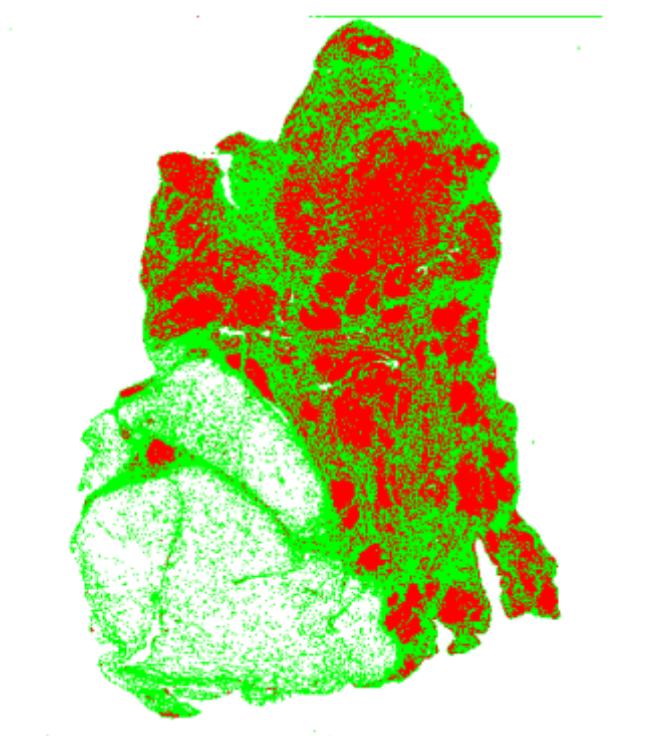
\includegraphics[scale=0.37]{images/TCGA-BH-A1FE-noback.png}
        \caption{Binary prediction map - red areas represent potential malignancy and green areas represent healthy tissue}
        \label{fig:binary-map}
    \end{subfigure}\hfill%
    ~~
    \begin{subfigure}[b]{0.4\textwidth}
        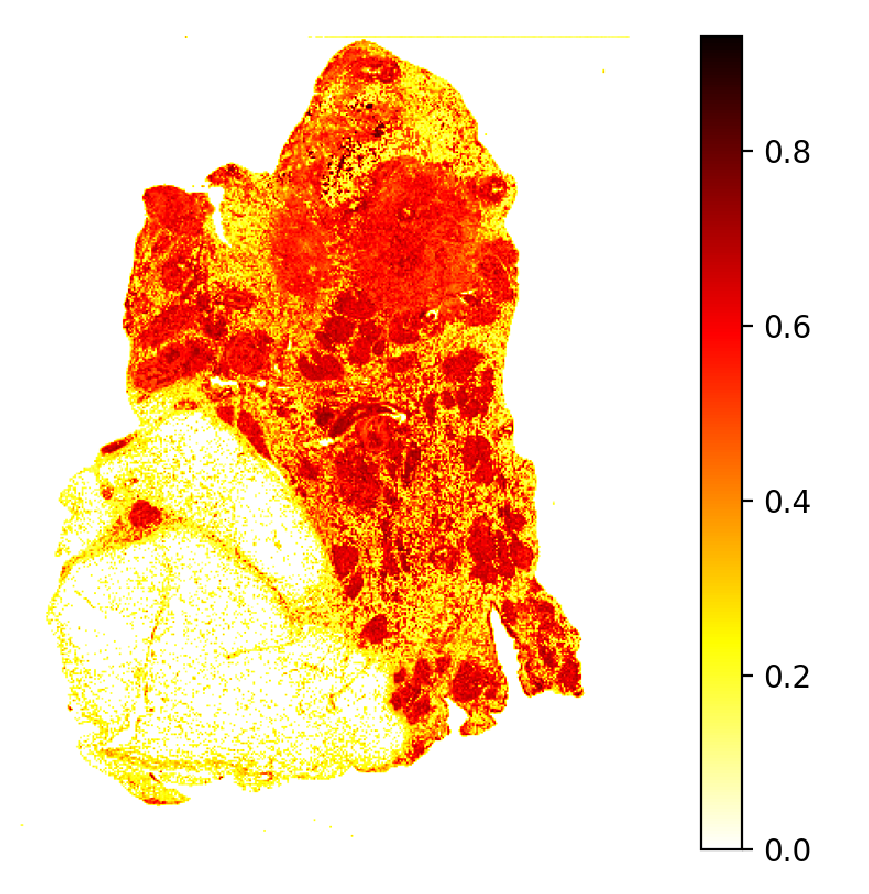
\includegraphics[scale=0.3]{images/TCGA-BH-A1FE-continuous.png}
        \caption{Continuous prediction heatmap - Darker areas represent regions of strong malignant intensity while lighter regions show lower malignant intensity/healthy tissue}
        \label{fig:continuous-heatmap}
    \end{subfigure}

    \caption{We illustrate the two types of feature maps generated during the prediction stage by our trained model. }
    \label{fig:visualization-example}
\end{figure}

\subsection{Regression model fitting}
 As described in section \ref{survival-analysis-methods}, we use the Lifelines Python package to develop our survival time estimation models. We first calculated the scores as illustrated in the previous section from the two types of feature predictions for each WSI in the feature extraction dataset. The calculated scores for each WSI was paired with the ground truth value of actual survival duration of the patient as retrieved from the associated clinical data available on CBioPortal \footnote{https://www.cbioportal.org/study/clinicalData?id=brca\_tcga\_pub2015\%2Cbrca\_tcga\%2Cbrca\_tcga\_pub\%2Cbrca\_tcga\_pan\_can\_atlas\_2018}.
\\
 \subsubsection{Cox Proportional Hazards Model}\hfill\\
We use the \texttt{CoxPHFitter} class from the Lifelines package to train a semi-parametric survival model using a dataset containing malignancy scores, survival duration and survival status of each patient. The Cox model uses the survival time of each patient as the duration parameter, the survival status as the event parameter and any other columns provided are used as covariates influencing survival hazard. Based on the input parameters, the Cox model develops a baseline hazard function. This is inferred as a change in population-level hazard over time given the occurrence of an event, i.e. the death of a subject in our case, at different points in time. Any individual patient's corresponding Log-hazard is then considered to be a linear function of their corresponding covariate value and this baseline generated by the Cox model as shown in equation \ref{eq:hazard model}. 
\\
\subsubsection{Survival time prediction}\hfill \\
We obtain two uni-variable Cox proportional hazard functions, each using one of the two malignancy features as hazard covariate in order to infer their individual impacts as a risk factor on patient survival. Finally, we used each model's \texttt{CoxPHFitter.predict\_median(covariate)} function, with computed value(s) of the corresponding model covariate provided as a parameter. This generated a median survival time prediction for the given score(s), in the same units as the training data, giving us an overall survival prognoses estimate for each patient. 

As shown in figure \ref{fig:KM-plot-result}, we have also generalized the model to show population level survival trends over time for a given covariate by using the \texttt{plot\_partial\_effects\_on\_outcome()} function. It generates Kaplan-Meier plots corresponding to each value provided, showing the covariate's exclusive effect on the survival probability of a cohort possessing that malignancy level, assuming all other factors remain constant. This probability decreases over time for all covariates indicating lower survival at later stages as metastases progresses accounting for no external factors like treatment. Furthermore,  The different covariate levels are plotted as graphs shifted around the baseline owing to the proportional nature of the Cox model as discussed in \ref{cph-background}. 

\begin{figure}[h]
    \centering
    \begin{subfigure}[b]{0.45\textwidth}
        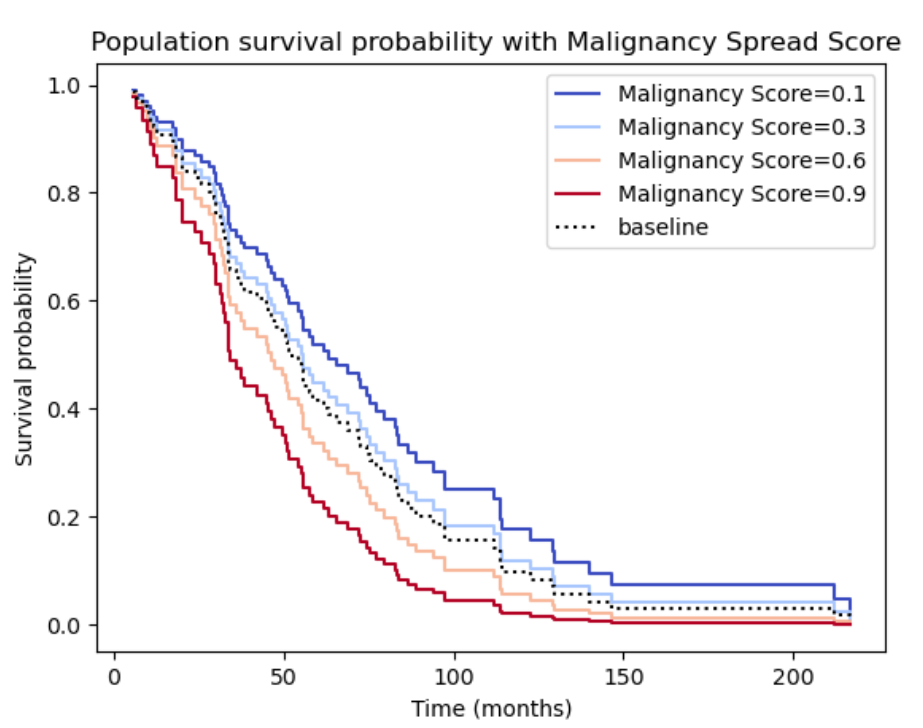
\includegraphics[scale=0.3]{images/binary-km.png}
        \caption{KM Plot of Malignancy Spread Score showing survival probability of patients with a score of 0.1, 0.3, 0.6 and 0.9 compared to the baseline survival. }
        \label{fig:binary-map}
    \end{subfigure}\hfill%
    ~
    \begin{subfigure}[b]{0.45\textwidth}
        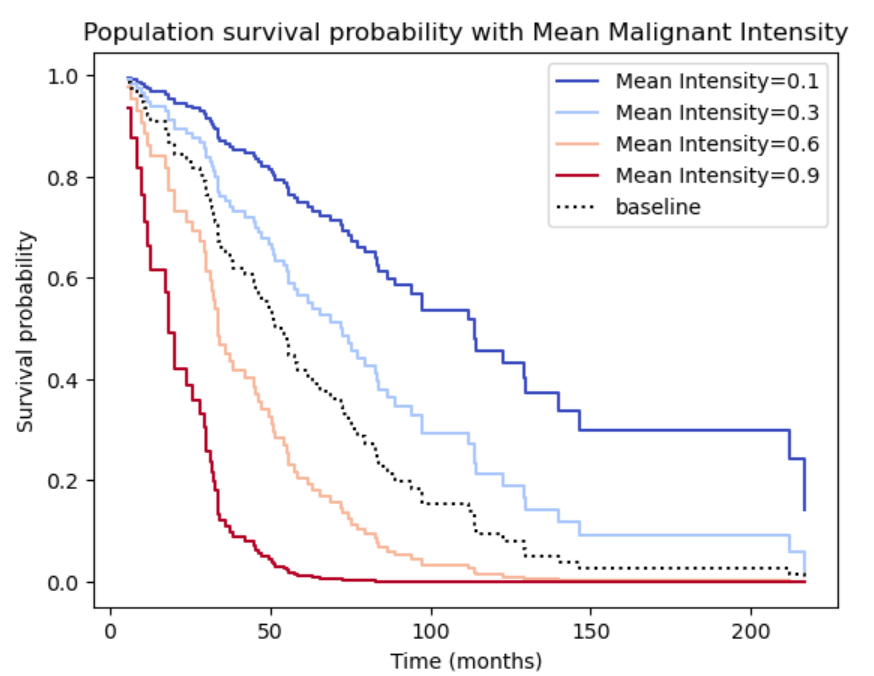
\includegraphics[scale=0.32]{images/continuous_km.png}
        \caption{KM Plot of Mean Malignant Intensity showing survival probability of patients with a score of 0.1, 0.3, 0.6 and 0.9 compared to the baseline survival.}
        \label{fig:continuous-heatmap}
    \end{subfigure}

    \caption{We illustrate the impact of the two covariates - Malignancy Spread Score and Mean Malignant Intensity - on survival probability over time with each curve corresponding to a different covariate level. Higher covariate values progressively shift the graph further below the baseline survival indicating lower overall survival in patients due to higher disease severity. This indicates a  Similarly, lower scores implying relatively less severe malignancy displays a graph above the baseline indicating reduced risk and higher survival probability.}
    \label{fig:KM-plot-result}
\end{figure}





%==================================================================================================================================
\chapter{Evaluation} 
\section{Classification stage - Cacncer detection}
\subsection{Classifier hyperparameter optimization}
The best model described in section \ref{cnn-architecture}, was developed with parameters determined by the results of hyperparameter tuning. We have investigated various configurations from the following hyperparameter space to identify the optimal model setting :
\begin{itemize}
    \item  activation function : tanh, relu, leaky relu
    \item dropout rate : \(p \in [0, 1)\)
    \item batch size : 32, 64, 128
    \item learning rate : \(lr \in \) [1e-5, 1e-1)
\end{itemize}

As described in section \ref{impl-hyperparam}, we first iteratively trained 20 random models sampled from the overall parameter space described above. Using loss and accuracy obtained from the validation dataset as our metric of choice, we identified the best model as highlighted in figure \ref{fig:tuning-stage-1}. The best model comprised of : TanH activation, 0.5 dropout, 0.001 learning rate, 64 training batch size and 32 validation batch size. The results indicated that models using TanH activation generally displayed the best performance overall, outperforming ReLU and Leaky ReLU by a significant margin. The batch sizes yielded the standard, expected value of 64 and 32 for an image classification problem implying they are not very consequential on the final metric. 

\begin{figure}[h]
    \centering
    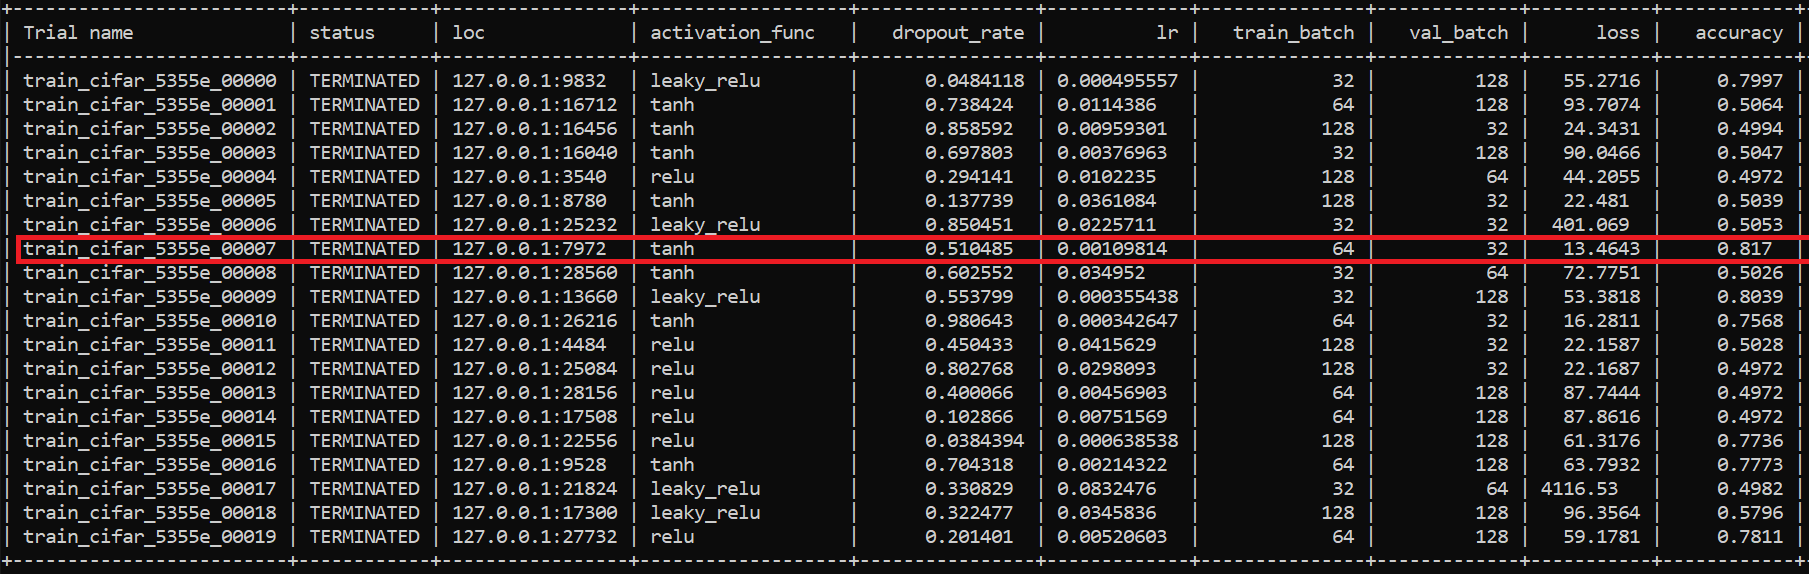
\includegraphics[scale=0.5]{images/tuning-stage1.png}
    \caption{Stage 1 Hyperparameter tuning results - Showing validation loss and accuracy values for 20 trained models with randomly sampled parameter settings. The best model with highest accuracy and lowest validation loss is highlighted in red. }
    \label{fig:tuning-stage-1}
\end{figure}

However, randomly sampling only 20 models did not allow us to fully explore the range of values chosen for learning rate and dropout. Due to us varying other parameters, there was some repetition observed in the values sampled for LR and Dropout across the 20 models causing a large range of values to remain unexplored. So we ran another tuning iteration with 10 models, this time keeping activation function and batch sizes fixed at the best setting obtained from the previous run and only sampling values for LR and Dropout. This allowed us to sample more unique values uniformly across the entire range of values specified above, yielding the final results as shown in figure \ref{fig:tuning-stage-2}

\begin{figure}[h]
    \centering
    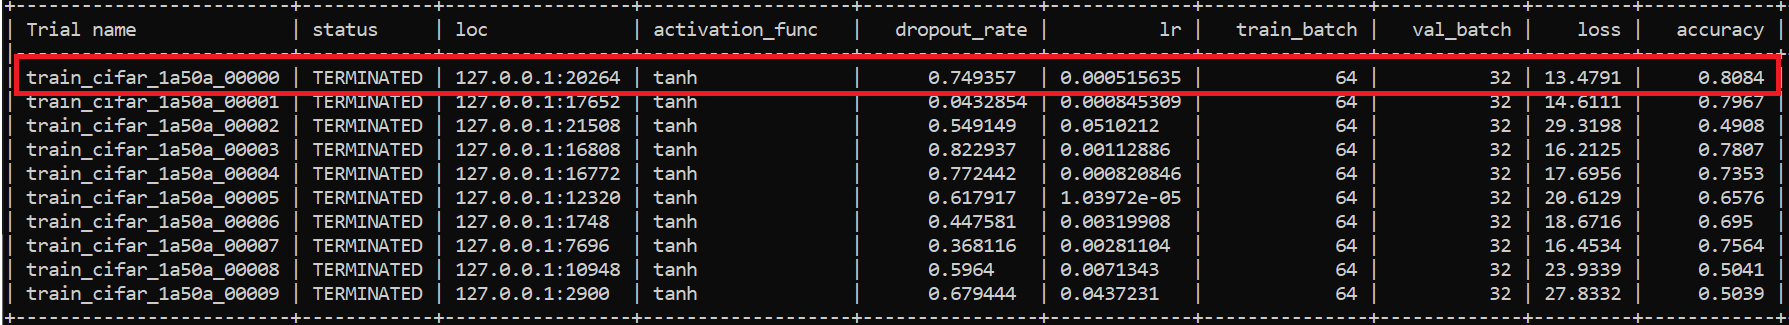
\includegraphics[scale=0.5]{images/tuning-stage2.png}
    \caption{Stage 2 Hyperparameter tuning results - Showing validation loss and accuracy values for 10 trained models with randomly sampled values for Learning Rate and Dropout while keeping Activation function and Batch sizes fixed to the value obtained in stage 1. }
    \label{fig:tuning-stage-2}
\end{figure}

As highlighted in figure \ref{fig:tuning-stage-2}, during the second iteration of hyperparameter tuning, a 0.75 Dropout and 0.0005 learning rate produced the best accuracy and lowest loss values when combined with the other parameters obtained in stage 1. The resulting model - TanH activation, 0.75 Dropout, 0.0005 LR and 64 training batch size was chosen as the final architecture, as described in section \ref{cnn-architecture}, for the classification task.

\subsection{Metrics for evaluating classification}
Our classification task predicts binary labels - malignant or benign - for each WSI tile. In order to measure the performance of our trained model we have chosen to use the standard metrics used in single-label classification - accuracy, precision and recall. We have processed a collection of 20,000 test images obtained from the PCAM dataset through our prediction pipeline to calculate these metrics for our model and also plot a \(2 \times 2\) confusion matrix to display the correctness of our prediction results. Using the concepts of true positives (TP), false positives (FP), true negatives (TN) and false negatives (FN) we calculated the metrics as follows:
\begin{itemize}
    \item \begin{equation}
        Accuracy = \frac{TP + TN}{TP + TN + FP + FN}
    \end{equation}

    \item \begin{equation}
        Recall = \frac{TP}{TP + FN}
    \end{equation}

    \item \begin{equation}
        Precision = \frac{TP}{TP + FP}
    \end{equation}
\end{itemize}

\subsection{How well does our deep learning model detect the presence of breast cancer from histopathology images?}
In figure \ref{fig:result-conf-mat}, we have illustrated our model's overall prediction results on the test dataset as a binary-class confusion matrix. This illustrates, that utilizing the model with the best parameter settings obtained after hyperparameter optimization, achieves significantly high overall performance. This is further evidenced in table \ref{tab:metric-data}, displaying the values obtained for our chosen metrics. Our model can distinguish between malignant and benign tiles with a 67\% accuracy indicating it is significantly better than a random model. However, it exhibits a 66\% precision in predicting malignant tiles. Given that our dataset is equally balanced, a completely random classifier would have displayed 50\% precision. Although this indicates that our model has actually learned something meaningful, it doesn't exhibit very high confidence in its predictions. Overall, the significant majority of all malignant predictions are likely to be relevant while only a small fraction of those predictions will be falsely labeled as malignant.

\begin{table}[h]
    \centering
    \begin{tabular}{c|c|c}
         Accuracy&Recall&Precision  \\ \hline
         0.67&0.74&0.66 
    \end{tabular}
    \caption{Computed scores for performance metrics - Accuracy, Recall and Precision - obtained from predictions generated on 20,000 PCAM test set images by the model with best parameters obtained from hyperparameter tuning.}
    \label{tab:metric-data}
\end{table}

We observe a fairly high recall score of 0.74 indicating our model is successfully detecting majority of all possible malignant tiles. When translated to the context of cancer characterization in a WSI, this would imply a slight underestimation of metastases severity as 26\% of actually malignant tiles are predicted as benign. As discussed in section \ref{cancer-general-problem}, a combination of abnormal nucleus growth and low cytoplasmic density indicate the presence of cancer. This makes detecting malignant tissue a lot more nuanced than detecting benign tissue. Our model often encounters cases where one or both of these metastases markers are present but not visually dominant in the tile causing the prediction to become biased towards the benign class. Considering random errors and variability in the quality of tissue slides, our model demonstrates high success in being able to significantly capture the overall extent of cancer in a given collection of tissue sections. 

\begin{figure}[h]
    \centering
    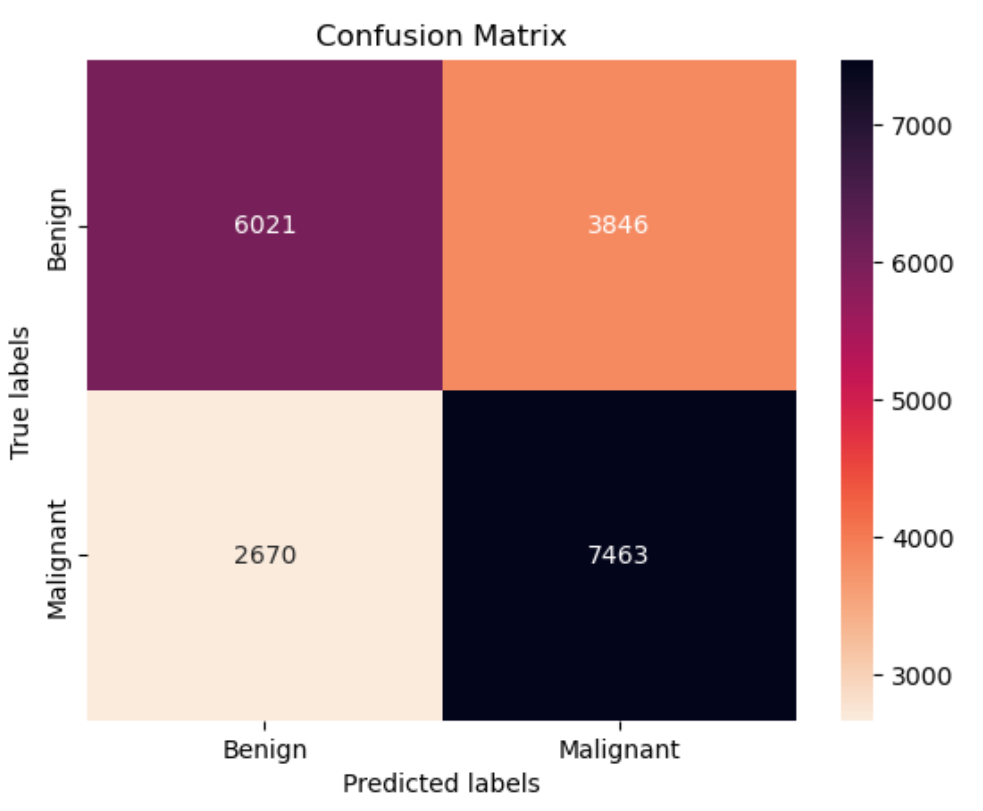
\includegraphics[scale=0.5]{images/confusion-matrix.png}
    \caption{Confusion matrix showing overall prediction performance of our best model when predicting classes for the PCAM test set images. Out of 20,000 query images - we have 10,133 malignant and 9867 benign tiles from which the model correctly predicts 7463 malignant and 6021 benign tiles.}
    \label{fig:result-conf-mat}
\end{figure}



\section{Regression stage - Survival prognosis prediction}
\subsection{Metrics for evaluating regression}
\subsection{How effectively does our survival model generate overall survival time predictions from extracted image features?}


% How good is your solution? How well did you solve the general problem, and what evidence do you have to support that?

% \section{Guidance}
% \begin{itemize}
%     \item
%         Ask specific questions that address the general problem.
%     \item
%         Answer them with precise evidence (graphs, numbers, statistical
%         analysis, qualitative analysis).
%     \item
%         Be fair and be scientific.
%     \item
%         The key thing is to show that you know how to evaluate your work, not
%         that your work is the most amazing product ever.
% \end{itemize}

% \section{Evidence}
% Make sure you present your evidence well. Use appropriate visualisations, reporting techniques and statistical analysis, as appropriate.

% If you visualise, follow the basic rules, as illustrated in Figure \ref{fig:boxplot}:
% \begin{itemize}
% \item Label everything correctly (axis, title, units).
% \item Caption thoroughly.
% \item Reference in text.
% \item \textbf{Include appropriate display of uncertainty (e.g. error bars, Box plot)}
% \item Minimize clutter.
% \end{itemize}

% See the file \texttt{guide\_to\_visualising.pdf} for further information and guidance.

% \begin{figure}
%     \centering
%     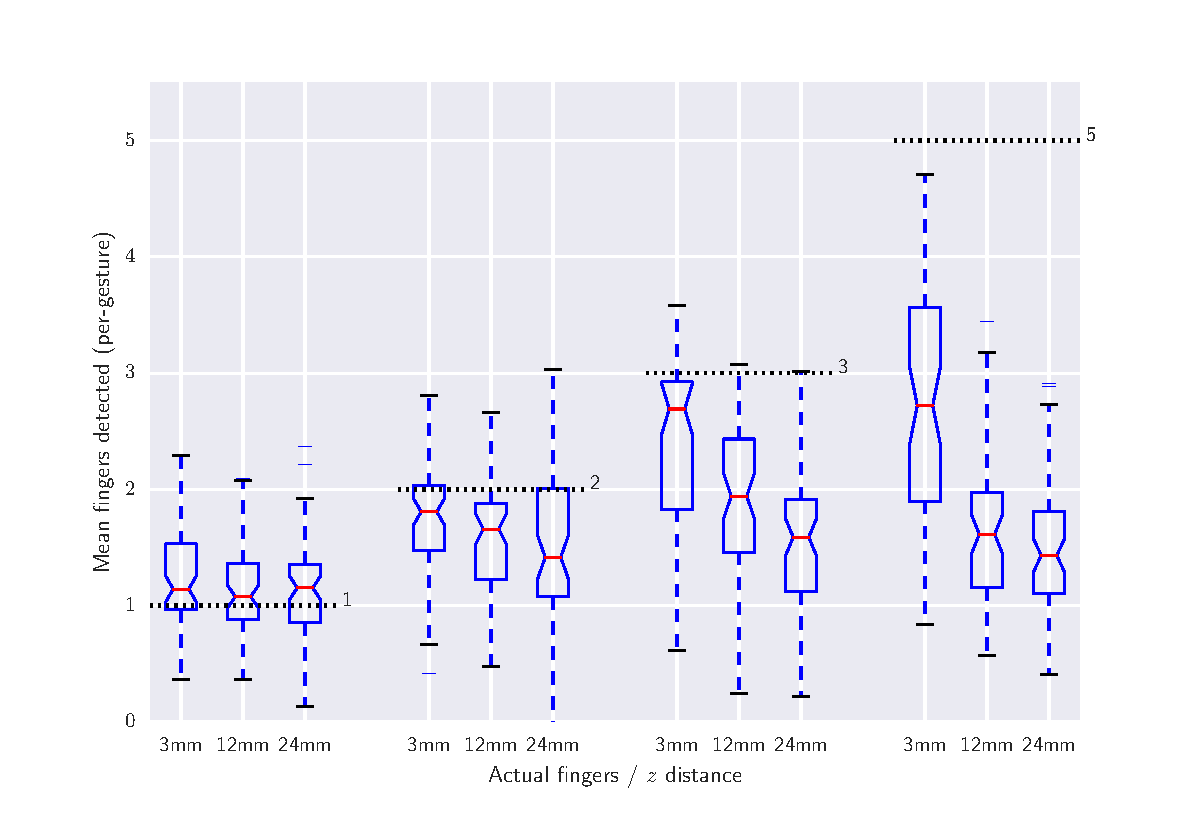
\includegraphics[width=1.0\linewidth]{images/boxplot_finger_distance.pdf}    

%     \caption{Average number of fingers detected by the touch sensor at different heights above the surface, averaged over all gestures. Dashed lines indicate
%     the true number of fingers present. The Box plots include bootstrapped uncertainty notches for the median. It is clear that the device is biased toward 
%     undercounting fingers, particularly at higher $z$ distances.
%     }

%     % use the notation fig:name to cross reference a figure
%     \label{fig:boxplot} 
% \end{figure}


%==================================================================================================================================
\chapter{Conclusion}    
Summarise the whole project for a lazy reader who didn't read the rest (e.g. a prize-awarding committee).
\section{Guidance}
\begin{itemize}
    \item
        Summarise briefly and fairly.
    \item
        You should be addressing the general problem you introduced in the
        Introduction.        
    \item
        Include summary of concrete results (``the new compiler ran 2x
        faster'')
    \item
        Indicate what future work could be done, but remember: \textbf{you
        won't get credit for things you haven't done}.
\end{itemize}

%==================================================================================================================================
%
% 
%==================================================================================================================================
%  APPENDICES  

\begin{appendices}

\chapter{Appendices}

Typical inclusions in the appendices are:

\begin{itemize}
\item
  Copies of ethics approvals (required if obtained)
\item
  Copies of questionnaires etc. used to gather data from subjects.
\item
  Extensive tables or figures that are too bulky to fit in the main body of
  the report, particularly ones that are repetitive and summarised in the body.

\item Outline of the source code (e.g. directory structure), or other architecture documentation like class diagrams.

\item User manuals, and any guides to starting/running the software.

\end{itemize}

\textbf{Don't include your source code in the appendices}. It will be
submitted separately.

\end{appendices}

%==================================================================================================================================
%   BIBLIOGRAPHY   

% The bibliography style is abbrvnat
% The bibliography always appears last, after the appendices.

\bibliographystyle{apalike}

\bibliography{l4proj}

\end{document}
